% ============================================================================
% 【最重要：本笔记的协作规则——每次编辑前请先读这里】
% ============================================================================
% 1. 默认只做：整理用户给出的 LaTeX 片段，并写入本文件，逐段推进。
% 2. 每轮写入后直接编译，并把生成的 PDF 提供给用户。
%    编译成功后不主动检查成品或渲染预览；编译失败时可以检查日志、排查并修复编译问题。
%    根据编译返回状态告知成功或失败；用户明确要求检查时，可以检查相关成品。
% 用户输入中若有英文或缩写，写入正文时改成中文（LaTeX 命令、数学符号及人名除外）。
% 人名保留原文，不译成汉语。
% 3. 最高优先级的编辑原则：几乎不修改用户上传的文字，只整理成能编译的 LaTeX。
%    这是用户给自己看的笔记，可以采用意会式、非严格的叙述；不要改写成严谨教材。
%    保留原话、缩写、直观记法和省略，不润色内容，不主动扩写、重组或补充理论。
%    必要时可修正命令、括号、数学环境；用户因懒而写了一半的公式，可按原意补全。
%    图文明显不匹配时可做最小必要修正（例如调整区域标号），不要借此扩写内容。
%    即使看出数学文本中有 gap，也不要补：这些省略往往是用户刻意留下的。
%    不为填补 gap 添加新的一两句话、过渡解释、条件说明或证明步骤，即使很简单。
%    若用户没有明确给出 proof，不要主动添加证明环节。
% 4. 用户要求从原书复制一小段时，从同目录的
%    stein_real_analysis_chapters_1_2_3_6.tex 提取指定片段，
%    仅做适配本笔记环境所需的修改，不主动复制更多内容。
% 5. 排版沿用同目录 probability_notes_template.tex 的风格：
%    ctexbook，英文 Chapter / Contents，彩色定理标题，现有定理编号方式。
% 6. 本笔记从测度开始，逐步写到一般积分理论；以用户的内容为主。
% 7. 编辑后只需简短告知写入位置和必要的改动；不要自行启动额外工作。
% 8. 若用户明确指出某处待补充、尚未写完或留待后续，应在该处加入醒目的“尚未写完，待补充”提醒，沿用现有大号加粗红字、浅红底和红色边框的样式；提醒文字按具体位置填写。
% 【再次强调：整理代码 + 写入 + 编译并提供 PDF；编译失败时允许检查和修复，成功后不主动检查成品。】
% ============================================================================
% !TeX program = xelatex
% 概率论讲义排版模板（按原 PDF 风格近似复刻）
\documentclass[12pt,letterpaper,twoside,openright]{ctexbook}

% 原 PDF 的中文正文字体为 FandolSong，西文/数学主要为 Latin Modern。
\usepackage{lmodern}
\usepackage[left=2cm,right=2cm,top=3.2cm,bottom=3.2cm]{geometry}
\usepackage{amsmath,amssymb,amsthm}
\usepackage{mathrsfs}
\usepackage{tikz}
\usepackage{xcolor}
\usepackage{hyperref}

% -------------------- 超链接 --------------------
% 原 PDF 目录条目为蓝色可点击链接，而页码保持黑色。
\hypersetup{
  colorlinks=true,
  linkcolor=blue,
  citecolor=blue,
  urlcolor=blue,
  linktoc=section
}

% -------------------- 章节样式 --------------------
% 保留英文 Chapter 1 / Contents 的外观。
\renewcommand{\contentsname}{Contents}
\ctexset{
  chapter = {
    name = {Chapter\ ,},
    number = \arabic{chapter},
    format = \raggedright\normalfont,
    nameformat = \huge,
    numberformat = \huge,
    titleformat = \Huge\bfseries,
    aftername = {\par\vspace{0.9em}},
    beforeskip = 10pt,
    afterskip = 26pt
  },
  section = {
    format = \raggedright\Large\bfseries,
    aftername = \quad,
    beforeskip = 3.2ex plus 1ex minus .2ex,
    afterskip = 1.5ex plus .2ex
  }
}

% book/ctexbook 的 headings 页眉与原 PDF 很接近：
% 偶数页：页码在左，章标题在右；奇数页：节标题在左，页码在右。
\pagestyle{headings}

% -------------------- 定理类环境 --------------------
% 原 PDF 中 theorem/proposition/corollary 共用一个全局编号；
% definition 自己全局编号；example 自己全局编号。
% 环境标题与正文同为 12pt，标题加粗并着色。

\newtheoremstyle{bluehead}
  {0.8\baselineskip}      % Space above
  {0.45\baselineskip}     % Space below
  {\normalfont}           % Body font
  {0pt}                    % Indent
  {\color{blue}\bfseries} % Head font
  {}                       % Punctuation after head
  {0.45em}                 % Space after head
  {\thmname{#1}\thmnumber{ #2.}\thmnote{(#3)}}

\newtheoremstyle{olivehead}
  {0.8\baselineskip}
  {0.45\baselineskip}
  {\normalfont}
  {0pt}
  {\color{olive}\bfseries}
  {}
  {0.45em}
  {\thmname{#1}\thmnumber{ #2.}\thmnote{(#3)}}

\newtheoremstyle{orangehead}
  {0.8\baselineskip}
  {0.45\baselineskip}
  {\normalfont}
  {0pt}
  {\color{orange}\bfseries}
  {}
  {0.45em}
  {\thmname{#1}\thmnumber{ #2.}\thmnote{(#3)}}

\newtheoremstyle{redremark}
  {0.8\baselineskip}
  {0.45\baselineskip}
  {\normalfont}
  {0pt}
  {\color{red}\bfseries}
  {}
  {0.45em}
  {\thmname{#1.}\thmnote{ (#3)}}

\theoremstyle{bluehead}
\newtheorem{theorem}{Theorem}
\newtheorem{proposition}[theorem]{Proposition}
\newtheorem{lemma}[theorem]{Lemma}
\newtheorem{corollary}[theorem]{Corollary}
% 原讲义中有 **Theorem、**Proposition 这样的强调写法。
\newtheorem{doubletheorem}[theorem]{**Theorem}
\newtheorem{doubleproposition}[theorem]{**Proposition}

\theoremstyle{olivehead}
\newtheorem{definition}{Definition}
% 原讲义中有 *Definition 这样的强调写法。
\newtheorem{stardefinition}[definition]{*Definition}

\theoremstyle{orangehead}
\newtheorem{example}[theorem]{Example}

\theoremstyle{redremark}
\newtheorem*{remark}{Remark}
\newtheorem*{observation}{Observation}

% amsthm 默认 Proof. 为斜体，结尾为方框，与原 PDF 基本一致。
\renewcommand{\proofname}{Proof}

% -------------------- 文档 --------------------
\begin{document}

\tableofcontents

\chapter{测度}

\section{测度}

\begin{definition}[代数]
设 $X$ 为一个集合。$X$ 的一个子集族 $\mathcal{P}$ 称为 $X$ 上的一个\textbf{代数}，如果它满足：
\begin{enumerate}
  \item $X \in \mathcal{P}$；
  \item 若 $A \in \mathcal{P}$，则 $X \setminus A \in \mathcal{P}$；
  \item （有限并的封闭性）若 $A_k \in \mathcal{P}$，$k=1,2,\ldots,n$，则
  \[
    \bigcup_{k=1}^{n} A_k \in \mathcal{P}.
  \]
\end{enumerate}
\end{definition}

\begin{definition}[$\sigma$-代数]
设 $X$ 为一个集合。$X$ 的一个子集族 $\mathcal{P}$ 称为 $X$ 上的一个\textbf{$\sigma$-代数}，如果它首先是一个代数，并且满足：
\begin{enumerate}
  \setcounter{enumi}{2}
  \item （可数并的封闭性）若 $A_n \in \mathcal{P}$，$n \in \mathbb{Z}_{>0}$，则
  \[
    \bigcup_{n=1}^{\infty} A_n \in \mathcal{P}.
  \]
\end{enumerate}
此时称 $(X,\mathcal{P})$ 为一个\textbf{可测空间}。
\end{definition}
\begin{remark}
注意：同一集合 $X$ 上任意非空族的 $\sigma$-代数的交仍是 $X$ 上的一个 $\sigma$-代数。这引出了如下定义。
\end{remark}

\begin{definition}[生成的 $\sigma$-代数]
设 $\mathcal{P}'$ 为集合 $X$ 的一个子集族。存在一个包含 $\mathcal{P}'$ 的最小的 $\sigma$-代数 $\mathcal{P}$，即
\[
  \mathcal{P}' \subseteq \mathcal{P},
\]
且对任意包含 $\mathcal{P}'$ 的 $\sigma$-代数 $\mathcal{Q}$，均有 $\mathcal{P} \subseteq \mathcal{Q}$。
称 $\mathcal{P}$ 为\textbf{由 $\mathcal{P}'$ 生成的 $\sigma$-代数}，记为 $\sigma(\mathcal{P}')$。
\end{definition}
\begin{definition}[测度空间]
设 $(X,\mathcal{P})$ 为一个可测空间。一个函数
\[
  \mu\colon \mathcal{P} \longrightarrow [0,+\infty]
\]
称为 $\mathcal{P}$ 上的一个\textbf{测度}，如果 $\mu(\varnothing)=0$，并且满足\textbf{可数可加性}：若 $E_i\in\mathcal{P}$，$i=1,2,\ldots$，且这些集合两两不交，即 $E_i\cap E_j=\varnothing$（$i\ne j$），则
\[
  \mu\!\left(\bigcup_{i=1}^{\infty} E_i\right)
  = \sum_{i=1}^{\infty} \mu(E_i).
\]
此时称 $(X,\mathcal{P},\mu)$ 为一个\textbf{测度空间}。
\end{definition}
\begin{remark}[\textrm{$\sigma$-有限性}]
若存在 $M_n\in\mathcal{P}$，$n=1,2,\ldots$，使得
\[
  X=\bigcup_{n=1}^{\infty}M_n,
  \qquad \mu(M_n)<\infty \quad (n=1,2,\ldots),
\]
则称测度空间 $(X,\mathcal{P},\mu)$ 是\textbf{$\sigma$-有限的}。
\end{remark}
注意：并非每个测度空间都是 $\sigma$-有限的。

\begin{example}
设 $X$ 为一个可数集合。给每个元素 $x\in X$ 赋予一个非负数 $a_x$，并对任意 $S\subseteq X$ 定义
\[
  \mu(S)=\sum_{x\in S}a_x.
\]
则 $\mu$ 是 $(X,2^X)$ 上的一个测度。
\end{example}
\begin{definition}[外测度]
设 $X$ 为一个集合。一个函数
\[
  \mu_*\colon 2^X\longrightarrow[0,+\infty]
\]
称为 $X$ 上的一个\textbf{外测度}，如果 $\mu_*(\varnothing)=0$，并且满足：
\begin{enumerate}
  \item （单调性）若 $E\subseteq F\subseteq X$，则 $\mu_*(E)\leq\mu_*(F)$；
  \item （可数次可加性）对任意 $E_i\subseteq X$，$i\in\mathbb{Z}_{>0}$，有
  \[
    \mu_*\!\left(\bigcup_{i=1}^{\infty}E_i\right)
    \leq\sum_{i=1}^{\infty}\mu_*(E_i).
  \]
\end{enumerate}
\end{definition}

\begin{definition}[预测度]
设 $\mathcal{A}$ 为 $X$ 上的一个代数。预测度是一个仅定义在 $\mathcal{A}$ 上的函数
\[
  \mu_0\colon\mathcal{A}\longrightarrow[0,+\infty],
\]
满足 $\mu_0(\varnothing)=0$，并且满足以下条件：
若 $E_i\in\mathcal{A}$，$i\in\mathbb{Z}_{>0}$，这些集合两两不交，且 $\bigcup_{i=1}^{\infty}E_i\in\mathcal{A}$，则
\[
  \mu_0\!\left(\bigcup_{i=1}^{\infty}E_i\right)
  =\sum_{i=1}^{\infty}\mu_0(E_i).
\]
\end{definition}
\begin{theorem}[外测度给出测度]\label{thm:outer-measure-construction}
设 $\mu_*$ 为集合 $X$ 上的一个外测度，令
\[
  \mathcal{M}=\left\{E\subseteq X\;\middle|\;
    \mu_*(A)=\mu_*(E\cap A)+\mu_*\bigl((X\setminus E)\cap A\bigr)
    \forall A\subseteq X
  \right\}.
\]
则：
\begin{enumerate}
  \item $\mathcal{M}$ 是 $X$ 上的一个 $\sigma$-代数；
  \item $\mu_*$ 在 $\mathcal{M}$ 上的限制 $\mu_*|_{\mathcal{M}}$ 是一个测度。
\end{enumerate}
\end{theorem}
\begin{observation}
\begin{enumerate}
  \item 在上述外测度的语境下，要证明集合 $E\subseteq X$ 是可测的，只需对任意 $A\subseteq X$ 证明
  \[
    \mu_*(A)\geq\mu_*(E\cap A)+\mu_*\bigl((X\setminus E)\cap A\bigr),
  \]
  因为反向不等式由外测度的可数次可加性保证。
  \item 外测度为零的集合是可测的，且其测度为零。
\end{enumerate}
\end{observation}

\begin{proof}
\textup{(1)} $\mathcal{M}$ 是一个 $\sigma$-代数。

难点在于证明可数并的封闭性。

\textbf{步骤 1.} 证明有限并的情形。注意，这可以归约到两个集合的并的情形。设 $E_1,E_2\in\mathcal{M}$，希望对任意 $A\subseteq X$ 证明
\[
  \mu_*(A)\geq
  \mu_*\bigl((E_1\cup E_2)\cap A\bigr)
  +\mu_*\bigl((X\setminus(E_1\cup E_2))\cap A\bigr).
\]
\medskip
\noindent
\begin{minipage}[c]{0.60\textwidth}
如右图，把 $A$ 的四个区域记为 $p,q,r,s$。为简洁起见，$pq$ 表示 $p\cup q$，$pqr$、$pqrs$ 等同理。要证明的就是
\[
  \mu_*(pqrs)\geq\mu_*(pqr)+\mu_*(s).
\]
实际上，由 $E_1,E_2$ 的可测性，
\[
\begin{aligned}
  \mu_*(pqrs)&=\mu_*(pq)+\mu_*(rs)\\
  &=\mu_*(p)+\mu_*(q)+\mu_*(r)+\mu_*(s)\\
  &\geq\mu_*(pqr)+\mu_*(s).
\end{aligned}
\]
最后一步用的是次可加性。
\end{minipage}\hfill
\begin{minipage}[c]{0.36\textwidth}
\centering
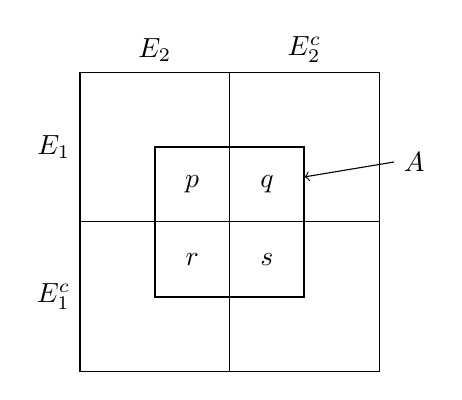
\begin{tikzpicture}[scale=0.95]
  \draw (0,0) rectangle (4,4);
  \draw (2,0)--(2,4) (0,2)--(4,2);
  \draw[thick] (1,1) rectangle (3,3);
  \node at (1,4.3) {$E_2$};
  \node at (3,4.3) {$E_2^c$};
  \node[left] at (0,3) {$E_1$};
  \node[left] at (0,1) {$E_1^c$};
  \node at (1.5,2.5) {$p$};
  \node at (2.5,2.5) {$q$};
  \node at (1.5,1.5) {$r$};
  \node at (2.5,1.5) {$s$};
  \node[right] at (4.2,2.8) {$A$};
  \draw[->] (4.2,2.8)--(3,2.6);
\end{tikzpicture}
\end{minipage}
\medskip

\textbf{步骤 2.} 对于可列个 $E_i\in\mathcal{M}$，令
\[
  G_n=\bigcup_{i=1}^{n}E_i,
  \qquad G=\bigcup_{n=1}^{\infty}G_n.
\]
由步骤 1，$G_n\in\mathcal{M}$，我们希望证明 $G\in\mathcal{M}$。
这是一个标准的技巧：先把集合变成递增的，再将其分成互不相交的层。

对任意 $A\subseteq X$，希望证明
\[
  \mu_*(A)\geq\mu_*(G\cap A)+\mu_*(A\setminus G).
\]
令 $G_0=\varnothing$，并记
\[
  a_i=A\cap(G_i\setminus G_{i-1}),\qquad b=A\setminus G.
\]
于是 $A\cap G=\bigcup_{i=1}^{\infty}a_i$，示意如下（图中的 $b_i$ 表示相应层内不属于 $A$ 的部分）：
\begin{center}
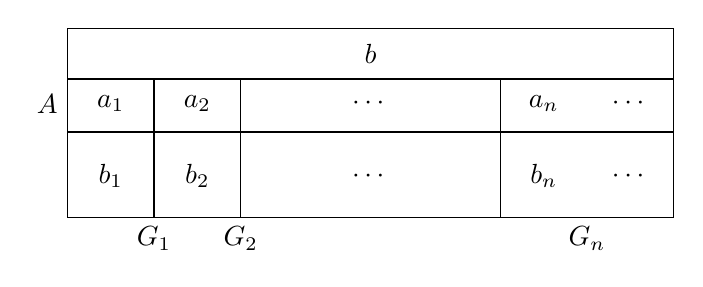
\begin{tikzpicture}[x=1.1cm,y=0.8cm]
  \draw (0,0) rectangle (7,3);
  \draw[thick] (0,1.35)--(7,1.35) (0,2.2)--(7,2.2);
  \foreach \x in {1,2,5} {\draw (\x,0)--(\x,2.2);}
  \node[left] at (0,1.8) {$A$};
  \node at (3.5,2.6) {$b$};
  \node at (0.5,1.8) {$a_1$};
  \node at (1.5,1.8) {$a_2$};
  \node at (3.5,1.8) {$\cdots$};
  \node at (5.5,1.8) {$a_n$};
  \node at (6.5,1.8) {$\cdots$};
  \node at (0.5,0.65) {$b_1$};
  \node at (1.5,0.65) {$b_2$};
  \node at (3.5,0.65) {$\cdots$};
  \node at (5.5,0.65) {$b_n$};
  \node at (6.5,0.65) {$\cdots$};
  \node[below] at (1,0) {$G_1$};
  \node[below] at (2,0) {$G_2$};
  \node[below] at (6,0) {$G_n$};
\end{tikzpicture}
\end{center}
由 $G_n\in\mathcal{M}$，并逐层利用可测性分割，得到
\[
\begin{aligned}
  \mu_*(A)
  &=\mu_*(A\cap G_n)+\mu_*(A\setminus G_n)\\
  &\geq\mu_*(A\cap G_n)+\mu_*(b)\\
  &=\sum_{i=1}^{n}\mu_*(a_i)+\mu_*(b).
\end{aligned}
\]
令 $n\to\infty$，再用可数次可加性，便有
\[
  \mu_*(A)\geq\sum_{i=1}^{\infty}\mu_*(a_i)+\mu_*(b)
  \geq\mu_*(A\cap G)+\mu_*(A\setminus G).
\]
因此 $G\in\mathcal{M}$。
% 后续证明由用户继续提供。
\end{proof}
\begin{theorem}[预测度扩展为外测度]
设 $\mu_0$ 是 $X$ 上的代数 $\mathcal{A}$ 上的一个预测度。在 $X$ 的子集上定义 $\mu_*$：
\[
  \mu_*(E)=\inf\left\{
    \sum_{j=1}^{\infty}\mu_0(E_j)\;\middle|\;
    E_j\in\mathcal{A},\quad E\subseteq\bigcup_{j=1}^{\infty}E_j
  \right\}.
\]
可以验证：
\begin{enumerate}
  \item $\mu_*$ 是 $X$ 上的一个外测度；
  \item $\mu_*(E)=\mu_0(E)$，$\forall E\in\mathcal{A}$；
  \item $\mathcal{A}$ 中所有集合在定理~\ref{thm:outer-measure-construction} 的语境下都是可测的。
\end{enumerate}
\end{theorem}
\begin{proof}
证明 \textup{(1)} 基本没有困难，只要合理使用 $\inf$ 的定义。

对于 \textup{(2)}，设 $E\in\mathcal{A}$，则 $E$ 覆盖自身，故
\[
  \mu_*(E)\leq\mu_0(E).
\]
希望证明：$\mu_*(E)\geq\mu_0(E)$。关键：只要证明总是有
\[
  \sum_{j=1}^{\infty}\mu_0(E_j)\geq\mu_0(E)
\]
即可，而不用管 $\mu_*(E)$。

对于 $E\subseteq\bigcup_{j=1}^{\infty}E_j$，使用标准技巧，不妨 $E_j\subseteq E_{j+1}$。
由预测度的定义（记 $E_0=\varnothing$），
\[
  \mu_0(E)
  =\sum_{j=1}^{\infty}\mu_0\bigl((E_j\setminus E_{j-1})\cap E\bigr)
  \leq\sum_{j=1}^{\infty}\mu_0(E_j\setminus E_{j-1}).
\]
对于 \textup{(3)}，设 $A\subseteq X$，$E\in\mathcal{A}$。希望证明
\[
  \mu_*(A)\geq\mu_*(E\cap A)+\mu_*(E^c\cap A).
\]
由定义，设 $A\subseteq\bigcup_{j=1}^{\infty}E_j$，$E_j\in\mathcal{A}$，则
\[
\begin{aligned}
  \sum_{j=1}^{\infty}\mu_0(E_j)
  &\geq\sum_{j=1}^{\infty}\mu_0(E\cap E_j)
      +\sum_{j=1}^{\infty}\mu_0(E^c\cap E_j)\\
  &\geq\mu_*(E\cap A)+\mu_*(E^c\cap A).
\end{aligned}
\]
对 $\{E_j\}$ 取下确界，得
\[
  \mu_*(A)\geq\mu_*(E\cap A)+\mu_*(E^c\cap A).
\]
\end{proof}
\begin{remark}
由定理~\ref{thm:outer-measure-construction}，可测集族是一个 $\sigma$-代数，所以有如下流程：
\begin{center}
\begin{tikzpicture}
  \node (pre) at (0,0) {$\mu_0$};
  \node (outer) at (5,0) {$\mu_*$};
  \node (measure) at (10,0) {$\mu$};
  \draw[->] (pre)--(outer);
  \draw[->] (outer)--(measure);
  \node[align=center,text width=3.5cm,anchor=north] at (0,-0.55)
    {$\mathcal{A}$ 上的预测度};
  \node[align=center,text width=3.5cm,anchor=north] at (5,-0.55)
    {$2^X$ 上的外测度};
  \node[align=center,text width=4cm,anchor=north] at (10,-0.55)
    {包含 $\mathcal{A}$ 的\\$\sigma$-代数上的测度};
\end{tikzpicture}
\end{center}
\end{remark}
\begin{theorem}[唯一性]\label{thm:measure-extension-uniqueness}
继续上文记号。若 $\mu_0$ 是 $\sigma$-有限的，则 $\sigma(\mathcal{A})$ 上与 $\mu_0$ 在 $\mathcal{A}$ 上一致的测度唯一，即为之前构造的 $\mu$ 在 $\sigma(\mathcal{A})$ 上的限制。
\end{theorem}
\begin{proof}
假设 $p$ 是另一个相容的、定义在包含 $\mathcal{A}$ 的最小 $\sigma$-代数上的测度。

\textbf{第一部分.} $p(F)\leq\mu(F)$。这是简单的，选择一个 $F$ 的 $\mathcal{A}$-覆盖即可。

\textbf{第二部分.} $p(F)\geq\mu(F)$。

对于 $\mu(F)<\infty$，设 $F\subseteq\bigcup_{j=1}^{\infty}E_j$，$E_j\in\mathcal{A}$。令 $E=\bigcup_{j=1}^{\infty}E_j$（不一定属于 $\mathcal{A}$）。有
\[
\begin{aligned}
  p(E)
  &=\lim_{n\to\infty}p\!\left(\bigcup_{j=1}^{n}E_j\right)
    \quad\text{（由测度定义）}\\
  &=\lim_{n\to\infty}\mu\!\left(\bigcup_{j=1}^{n}E_j\right)
  =\mu(E).
\end{aligned}
\]
对于 $E$，设 $\mu(E)\leq\mu(F)+\varepsilon$，则 $\mu(E\setminus F)\leq\varepsilon$，于是
\[
\begin{aligned}
  \mu(F)&\leq\mu(E)=p(E)\\
  &=p(F)+p(E\setminus F)\\
  &\leq p(F)+\mu(E\setminus F)\\
  &\leq\varepsilon+p(F).
\end{aligned}
\]
令 $\varepsilon\to0$ 即可。
对于 $\mu(F)=\infty$，这里要用到 $\sigma$-有限性。具体就是使用定义，并让 $F$ 和 $M_n$ 们取交即可。
\end{proof}
\begin{remark}
注意：预测度的 $\sigma$-有限性和扩张到 $2^X$ 上的外测度之后的 $\sigma$-有限性是等价的，与限制之后的测度的 $\sigma$-有限性也等价。

\end{remark}

\begin{definition}[完备性]
称测度空间 $(X,\mathcal{P},\mu)$ 是\textbf{完备的}，如果每个零测集的所有子集都是可测的，即若 $N\in\mathcal{P}$、$\mu(N)=0$ 且 $B\subseteq N$，则 $B\in\mathcal{P}$。
\end{definition}

\begin{remark}
外测度限制在全部可测集组成的 $\mathcal{M}$ 上，得到的测度是完备的。因为若 $B\subseteq N$ 且 $\mu_*(N)=0$，由单调性有 $\mu_*(B)=0$，所以 $B$ 可测。

从一个测度空间 $(X,\mathcal{P},\mu)$ 出发，把 $\mu$ 当作预测度，构造外测度 $\mu_*$，再限制到全部外测度可测集组成的 $\mathcal{M}$ 上，有
\[
  \mathcal{P}\subseteq\mathcal{M},\qquad\mu_*|_{\mathcal{P}}=\mu.
\]
原来可测集的测度不变，但定义域可能变大：$\mathcal{M}$ 包含原零测集的所有子集，这些子集原来未必在 $\mathcal{P}$ 中。

如果只限制回原来的 $\mathcal{P}$，就得到原来的测度，但不一定完备。限制到全部外测度可测集，与限制回原来的子集族，是两回事。
\end{remark}
\begin{definition}[可测函数]
设 $(X,\mathcal{P})$ 为一个可测空间。称函数 $f\colon X\to[-\infty,+\infty]$ 是\textbf{可测的}，假如对任何 $a\in\mathbb{R}$，
\[
  f^{-1}([-\infty,a))=\{x\in X\mid f(x)<a\}
\]
是可测集。
\end{definition}

% 以下摘自 Stein 第一章“可测函数”一节的 Property 3--6，仅列结论。
\begin{proposition}
设 $f$ 为取有限值的函数，则以下条件等价：
\begin{enumerate}
  \item $f$ 是可测的；
  \item 对任意 $a,b\in\mathbb{R}$，$a<b$，$f^{-1}((a,b))=\{x:a<f(x)<b\}$ 是可测集；
  \item 对任意开集 $O\subseteq\mathbb{R}$，$f^{-1}(O)$ 是可测集；
  \item 对任意闭集 $F\subseteq\mathbb{R}$，$f^{-1}(F)$ 是可测集。
\end{enumerate}
\end{proposition}
\begin{proposition}
设 $\{f_n\}_{n=1}^{\infty}$ 是一列可测函数，则
\[
  \sup_n f_n(x),\qquad\inf_n f_n(x),\qquad
  \limsup_{n\to\infty}f_n(x),\qquad
  \liminf_{n\to\infty}f_n(x)
\]
都是可测的。
\end{proposition}

\begin{proposition}
若 $\{f_n\}_{n=1}^{\infty}$ 是一列可测函数，且
\[
  \lim_{n\to\infty}f_n(x)=f(x),
\]
则 $f$ 是可测的。
\end{proposition}

\begin{proposition}
若 $f,g$ 是可测函数，则：
\begin{enumerate}
  \item 整数次幂 $f^k$，$k\geq1$，是可测的；
  \item 若 $f,g$ 都取有限值，则 $f+g$ 和 $fg$ 是可测的。
\end{enumerate}
\end{proposition}


\noindent 这些验证起来都比较简单。例如，
\begin{flalign*}
  &\{x:f(x)<a\}
  =\bigcup_{k=1}^{\infty}\bigcup_{N=1}^{\infty}\bigcap_{m=N}^{\infty}
  \left\{x:f_m(x)<a-\frac{1}{k}\right\}. &&
\end{flalign*}
\noindent 或者使用上面的 $\limsup$ 论证。
\begin{definition}[简单函数]
集合 $E$ 的特征函数定义为
\[
  \chi_E(x)=
  \begin{cases}
    1,&x\in E,\\
    0,&x\notin E.
  \end{cases}
\]
一个\textbf{简单函数}是有限和
\[
  f=\sum_{k=1}^{N}a_k\chi_{E_k},
\]
其中每个 $E_k$ 都是有限测度的可测集，$a_k$ 为常数。
\end{definition}
\begin{proposition}\label{prop:simple-function-approx}
设 $(X,\mathcal{P},\mu)$ 是一个 $\sigma$-有限测度空间，$f$ 是 $X$ 上的非负可测函数，则存在一列递增的非负简单函数 $\{\varphi_k\}_{k=1}^{\infty}$，逐点收敛到 $f$，即对所有 $x$，
\[
  \varphi_k(x)\leq\varphi_{k+1}(x),\qquad
  \lim_{k\to\infty}\varphi_k(x)=f(x).
\]
一般地，若 $f$ 是可测函数，则存在一列简单函数 $\{\varphi_k\}$，对所有 $x$ 满足
\[
  |\varphi_k(x)|\leq|\varphi_{k+1}(x)|,\qquad
  \lim_{k\to\infty}\varphi_k(x)=f(x).
\]\end{proposition}

\begin{proof}
首先作截断。由 $\sigma$-有限性，取有限测度的可测集 $Q_N\uparrow X$，定义
\[
  F_N(x)=
  \begin{cases}
    f(x),&x\in Q_N\text{ 且 }f(x)\leq N,\\
    N,&x\in Q_N\text{ 且 }f(x)>N,\\
    0,&\text{其他情形}.
  \end{cases}
\]
当 $N\to\infty$ 时，对所有 $x$ 都有 $F_N(x)\to f(x)$。现在分割 $F_N$ 的值域 $[0,N]$。对于固定的 $N,M\geq1$，定义
\[
  E_{\ell,M}=\left\{x\in Q_N:
    \frac{\ell}{M}<F_N(x)\leq\frac{\ell+1}{M}\right\},
  \qquad 0\leq\ell<NM.
\]
令
\[
  F_{N,M}(x)=\sum_{\ell=0}^{NM-1}\frac{\ell}{M}\chi_{E_{\ell,M}}(x).
\]
每个 $F_{N,M}$ 都是简单函数，且对所有 $x$，
\[
  0\leq F_N(x)-F_{N,M}(x)\leq\frac1M.
\]
取 $N=M=2^k$，其中 $k\geq1$ 为整数，并令 $\varphi_k=F_{2^k,2^k}$，则对所有 $x$，
\[
  0\leq F_{2^k}(x)-\varphi_k(x)\leq\frac1{2^k}.
\]
$\{\varphi_k\}$ 是递增的，并满足所需的全部性质。
对于一般的 $f$，将 $f=f^+-f^-$ 的正负部分分别用递增的非负简单函数 $\varphi_k^{(1)}$、$\varphi_k^{(2)}$ 逼近，令
\[
  \varphi_k=\varphi_k^{(1)}-\varphi_k^{(2)}.
\]
则 $\varphi_k\to f$，且 $|\varphi_k|=\varphi_k^{(1)}+\varphi_k^{(2)}$ 递增。\end{proof}
\begin{proposition}[简单函数的一致逼近]\label{prop:uniform-simple-approx}
设 $f$ 是测度空间 $(X,\mathcal M,\mu)$ 上的有界实值可测函数。$f$ 可以由一列简单函数一致逼近，当且仅当
\[
\mu\{x:|f(x)|>\varepsilon\}<\infty\qquad\text{对每个 }\varepsilon>0.
\]
\end{proposition}

\begin{proof}
充分性：把之前按空间截断改成按函数值大小截断。令 $A_n=\{|f|>1/n\}$，则 $\mu(A_n)<\infty$。在 $A_n$ 上分割有界值域，取简单函数 $s_n$，使误差不超过 $1/n$；在 $A_n^c$ 上令 $s_n=0$。于是 $\sup_X|f-s_n|\leq1/n$，且 $s_n$ 的支集测度有限。

必要性：若 $s_n\to f$ 一致，对任意 $\varepsilon>0$，取 $n$ 使 $\sup_X|f-s_n|<\varepsilon/2$，则
\[
\{|f|>\varepsilon\}\subseteq\{|s_n|>\varepsilon/2\}
\subseteq\operatorname{supp}s_n,
\]
所以该集合测度有限。
\end{proof}
\begin{remark}
这个命题不需要测度空间的 $\sigma$-有限性。$A_n=\{|f|>1/n\}$ 起到了原来递增的有限测度截断集的类似作用，但只需 $A_n\uparrow\{f\ne0\}$，不必覆盖整个 $X$；剩下的地方 $f=0$，让逼近函数也为零即可。
\end{remark}
\begin{theorem}[Egorov 定理]\label{thm:egorov-general}
设 $\{f_k\}$ 是定义在可测集 $E\subseteq X$ 上的一列可测函数，$\mu(E)<\infty$，且 $f_k\to f$ 几乎处处成立（即除去一个零测集后，$f_k(x)\to f(x)$）。则对任何 $\varepsilon>0$，存在 $E_\varepsilon\subseteq E$，使得
\[
  \mu(E\setminus E_\varepsilon)<\varepsilon,
\]
且 $f_k$ 在 $E_\varepsilon$ 上一致收敛到 $f$。
\end{theorem}
\begin{observation}
不妨设 $\lim_{n\to\infty}f_n=f$ 在 $E$ 上成立，而非仅几乎处处成立。
\end{observation}
\begin{proof}
令
\[
  g_N(x)=\sup_{n\geq N}|f_n(x)-f(x)|\qquad\text{（技巧）}。
\]
则 $\{g_N(x)\}$ 满足：可测、单调减、处处收敛到 $0$。

直观地，令
\[
  A_{n,N}=\left\{x\in E:g_N(x)<\frac1n\right\},
\]
则 $A_{n,N}$ 随 $n$ 逐渐变小，随 $N$ 逐渐变大（直到 $E$）。目标：
\[
  \bigcap_{n=1}^{\infty}A_{n,N_n},\qquad
  \lim_{n\to\infty}N_n=+\infty.
\]
所以这就说明显了：让每个 $n$ 都选择一个 $N_n$，使得 $A_{n,N_n}$ 充分大即可。最后一步用经典的 $\sum_{n=1}^{\infty}\varepsilon/2^n$ 规避 $\sum_{n=1}^{\infty}\varepsilon$。
\end{proof}
\section{积分}

\begin{definition}[积分]
对于可测函数 $f$ 和测度 $\mu$，假使 $X$ 是 $\sigma$-有限的，我们能定义积分
\[
  \int_X f\,d\mu.
\]
如果 $\int_X|f|\,d\mu<\infty$，则称 $f$ \textbf{可积}。
\end{definition}

下面来介绍 $\int_X f\,d\mu$ 的定义方式。

\textbf{步骤 1. 简单函数。} 若 $\varphi(x)=\sum_{k=1}^{N}a_k\chi_{E_k}(x)$，则定义
\[
  \int_X\varphi\,d\mu=\sum_{k=1}^{N}a_k\mu(E_k).
\]
易看出良定性。

我们从步骤 1 中提取“我们希望”积分具有的性质：
\begin{enumerate}
  \item[(1)] 线性：
  \[
    \int(af+bg)\,d\mu=a\int f\,d\mu+b\int g\,d\mu.
  \]
  \item[(2)] 可加性：设 $A,B$ 可测，$A\cap B=\varnothing$，则
  \[
    \int_{A\cup B}f\,d\mu=\int_A f\,d\mu+\int_B f\,d\mu.
  \]
  （注意，在 Riemann 积分中不对！）
  \item[(3)] 单调性。
  \item[(4)] 不等式：
  \[
    \left|\int f\,d\mu\right|\leq\int|f|\,d\mu.
  \]
  \item[(5)] 如果 $f,g$ 都是简单函数，且几乎处处相同，则
  \[
    \int f\,d\mu=\int g\,d\mu.
  \]
\end{enumerate}

\textbf{步骤 2. 有界函数。} $f$ 有界，$\operatorname{supp}f$ 的测度有限。

注意：这里暂时我们只能让
\[
  \operatorname{supp}f=\{x\in X:f(x)\ne0\},
\]
因为 $X$ 没有拓扑结构。

\begin{lemma}
$f$ 有界，$\mu(\operatorname{supp}f)<\infty$。设 $\{\varphi_n\}$ 是一列简单函数，且 $\varphi_n(x)\to f(x)$ 对几乎处处的 $x\in X$ 成立，则 $\lim_{n\to\infty}\int\varphi_n\,d\mu$ 存在，且如果 $f=0$ 几乎处处，则
\[
  \lim_{n\to\infty}\int\varphi_n\,d\mu=0.
\]
这里第二个命题能推出 $\lim_{n\to\infty}\int\varphi_n\,d\mu$ 的唯一性，从而可用作 $\int f\,d\mu$ 的定义。
\end{lemma}

\begin{proof}
注意：假如 $\varphi_n$ 一致收敛到 $f$，那结果是明显的。

主动使用 Egorov 定理：对于任意 $\varepsilon>0$，存在 $A_\varepsilon$，$\mu(E\setminus A_\varepsilon)<\varepsilon$，而 $\varphi_n$ 在 $A_\varepsilon$ 上一致收敛到 $f$。让 $|\varphi_n-\varphi_m|<\varepsilon$ 在 $A_\varepsilon$ 上恒成立，从而
\[
\begin{aligned}
  \left|\int\varphi_n\,d\mu-\int\varphi_m\,d\mu\right|
  &\leq\int|\varphi_n-\varphi_m|\,d\mu\\
  &\leq\int_{A_\varepsilon}|\varphi_n-\varphi_m|\,d\mu
    +\int_{E\setminus A_\varepsilon}|\varphi_n-\varphi_m|\,d\mu
    \quad\text{（由可加性）}\\
  &\leq\mu(E)\varepsilon+2M\varepsilon\longrightarrow0.
\end{aligned}
\]
由 Cauchy 准则即知收敛。对于第二个结论同理。
\end{proof}
注意：步骤 2 中的积分也有一样的性质，读者写出
\[
  \lim_{n\to\infty}\int\varphi_n\,d\mu=\int f\,d\mu
\]
即可看出。步骤 3、4 也一样。

\textbf{步骤 3. 非负函数。} 我们考虑 $f\geq0$，但 $f$ 不一定有界。令
\[
  \int f\,d\mu=\sup_{0\leq g\leq f}\int g\,d\mu,
\]
$g$ 是步骤 2 中允许的那类函数即可。

\textbf{步骤 4. 一般的函数。} 用经典分解 $f=f^+-f^-$ 即可。

\begin{proposition}
设 $f\geq0$ 为可测函数，则
\[
  \int_X f\,d\mu=0\quad\Longleftrightarrow\quad f=0\text{ 几乎处处}.
\]
\end{proposition}

\begin{proof}
仅须证明“$\Rightarrow$”：令 $E_n=\{x\in X:f(x)>1/n\}$，它们是零测集，则 $\bigcup_{n=1}^{\infty}E_n$ 是零测集。
\end{proof}
\begin{remark}
可测函数 $f$ 若几乎处处为 $0$，则一定可积，且 $\int_X f\,d\mu=0$。这不需要 $f\geq0$。
\end{remark}
\begin{proposition}
设 $f$ 在测度空间 $(X,\mathcal{P},\mu)$ 上可积。则对于每个 $\varepsilon>0$：
\begin{enumerate}
  \item[(1)] 存在有限测度的可测集 $B$，使得
  \[
    \int_{X\setminus B}|f|\,d\mu<\varepsilon.
  \]
  \item[(2)] 存在 $\delta>0$，使得对任意可测集 $E$，
  \[
    \mu(E)<\delta\quad\Longrightarrow\quad\int_E|f|\,d\mu<\varepsilon.
  \]
\end{enumerate}
最后一个性质称为绝对连续性。
\end{proposition}




\begin{theorem}[单调收敛定理]\label{thm:monotone-convergence}
设 $\{f_n\}$ 是一列非负可测函数，$f_n\uparrow f$，则
\[
  \lim_{n\to\infty}\int_X f_n\,d\mu=\int_X f\,d\mu.
\]
\end{theorem}
\begin{proof}
先对于步骤 2，即有界且支集测度有限的情况来证明。

对于 $n\in\mathbb{Z}_{>0}$，取简单函数 $\varphi_n$ 来一致逼近 $f_n$：对所有 $x$，
\[
  0\leq f_n(x)-\varphi_n(x)\leq2^{-n}.
\]
（具体如何证明可看 Proposition~\ref{prop:simple-function-approx}。）现在 $\varphi_n(x)\to f(x)$，所以
\[
  \lim_{n\to\infty}\int\varphi_n\,d\mu=\int f\,d\mu.
\]
另一方面，
\[
  \int\varphi_n\,d\mu\leq\int f_n\,d\mu\leq\int f\,d\mu,
\]
所以 $\lim_{n\to\infty}\int f_n\,d\mu=\int f\,d\mu$。

对于一般情形，回顾
\[
  \int f\,d\mu
  =\sup\left\{\int g\,d\mu:\ g\text{ 属于步骤 2 的情形},\ 0\leq g\leq f\right\}.
\]
令 $g_n=\min\{g,f_n\}$，则
\[
  \lim_{n\to\infty}\int g_n\,d\mu=\int g\,d\mu.
\]
而 $g_n\leq f_n$，所以
\[
  \int g\,d\mu\leq\lim_{n\to\infty}\int f_n\,d\mu.
\]
对 $g$ 取上确界，得到
\[
  \int f\,d\mu\leq\lim_{n\to\infty}\int f_n\,d\mu.
\]
而 $\int f_n\,d\mu\leq\int f\,d\mu$，所以
\[
  \int f\,d\mu=\lim_{n\to\infty}\int f_n\,d\mu.
\]
\end{proof}
\begin{corollary}
设 $f_n,f$ 是可测函数，$0\leq f_n\leq f$，且 $f_n\to f$ 几乎处处，则 $\int_X f_n\,d\mu\to\int_X f\,d\mu$。允许 $\int_X f\,d\mu=\infty$，不要求 $f_n$ 单调。
\end{corollary}

\begin{proof}
令 $g_n(x)=\inf_{k\geq n}f_k(x)$，则 $g_n$ 可测，$0\leq g_n\uparrow f$ 几乎处处，且 $g_n\leq f_n\leq f$。由\hyperref[thm:monotone-convergence]{单调收敛定理}，$\int_X g_n\,d\mu\to\int_X f\,d\mu$。再由 $\int_X g_n\,d\mu\leq\int_X f_n\,d\mu\leq\int_X f\,d\mu$，得到所需结论；当 $\int_X f\,d\mu=\infty$ 时，左端趋于无穷，中间也趋于无穷。
\end{proof}




\begin{theorem}[Fatou 引理]
若 $\{f_n\}$ 是 $X$ 上的一列非负可测函数，则
\[
  \int_X\liminf_{n\to\infty}f_n\,d\mu
  \leq\liminf_{n\to\infty}\int_X f_n\,d\mu.
\]
\end{theorem}
\begin{proof}
令
\[
  g_n(x)=\inf_{k\geq n}f_k(x).
\]
则每个 $g_n$ 都是非负可测函数，且
\[
  g_n\uparrow\liminf_{n\to\infty}f_n.
\]
由\hyperref[thm:monotone-convergence]{单调收敛定理}，
\[
  \int_X\liminf_{n\to\infty}f_n\,d\mu
  =\lim_{n\to\infty}\int_X g_n\,d\mu.
\]
另一方面，对任意 $k\geq n$，有 $g_n\leq f_k$，故
\[
  \int_X g_n\,d\mu\leq\inf_{k\geq n}\int_X f_k\,d\mu.
\]
令 $n\to\infty$，得到
\[
  \int_X\liminf_{n\to\infty}f_n\,d\mu
  \leq\lim_{n\to\infty}\inf_{k\geq n}\int_X f_k\,d\mu
  =\liminf_{n\to\infty}\int_X f_n\,d\mu.
\]
\end{proof}
\begin{remark}
考虑 $X=\mathbb{Z}_{>0}$，$a_i\geq0$ 是 $\{i\}$ 的测度。从而 Fatou 引理即
\[
  \sum_{i=1}^{\infty}a_i\liminf_{n\to\infty}f_n(i)
  \leq\liminf_{n\to\infty}\sum_{i=1}^{\infty}a_i f_n(i).
\]
这给出如下引理（合并 $f_n(i)$ 和 $a_i$）：对于数列 $A_{p,q}\geq0$，有
\[
  \sum_{q=1}^{\infty}\liminf_{p\to\infty}A_{p,q}
  \leq\liminf_{p\to\infty}\sum_{q=1}^{\infty}A_{p,q}.
\]
\end{remark}

\begin{theorem}[控制收敛定理]\label{thm:dominated-convergence}
若 $\{f_n\}$ 是一列可测函数，$f_n\to f$ 几乎处处成立，且对于某个可积函数 $g$，有 $|f_n|\leq g$，则
\[
  \int_X|f_n-f|\,d\mu\longrightarrow0,
\]
从而
\[
  \int_X f_n\,d\mu\longrightarrow\int_X f\,d\mu.
\]
\end{theorem}
\begin{proof}
令
\[
  h_n=2g-|f_n-f|.
\]
则
\[
  0\leq h_n\leq2g,\qquad h_n\to2g\quad\text{几乎处处}.
\]
由\hyperref[thm:monotone-convergence]{单调收敛定理}，
\[
  \int_X h_n\,d\mu\longrightarrow2\int_X g\,d\mu.
\]
由于 $\int_X g\,d\mu<\infty$，得到
\[
  \int_X|f_n-f|\,d\mu
  =2\int_X g\,d\mu-\int_X h_n\,d\mu\longrightarrow0.
\]
从而
\[
  \left|\int_X f_n\,d\mu-\int_X f\,d\mu\right|
  \leq\int_X|f_n-f|\,d\mu\longrightarrow0.
\]
\end{proof}
\section{乘积测度与 Fubini 定理}

\begin{definition}[乘积测度]
设 $(X_1,\mathcal{M}_1,\mu_1)$、$(X_2,\mathcal{M}_2,\mu_2)$ 是测度空间。考虑 $X=X_1\times X_2$ 中的可测矩形 $A\times B$，其中 $A\in\mathcal{M}_1$、$B\in\mathcal{M}_2$。

进一步考虑代数 $\mathcal{A}$：可测矩形的有限不交并。
在 $\mathcal{A}$ 上有自然的预测度：若
\[
  E=\bigcup_{j=1}^{n}(A_j\times B_j),
  \qquad\{A_j\times B_j\}_{j=1}^{n}\text{ 两两不交},
\]
则
\[
  \mu_0(E)=\sum_{j=1}^{n}\mu_1(A_j)\mu_2(B_j).
\]
这是良定的。从而可得 $\mathcal{A}$ 生成的 $\sigma$-代数上的测度，记该 $\sigma$-代数为 $\mathcal{M}$，所得测度称为\textbf{乘积测度}。
\end{definition}

\begin{definition}
对于 $E\in\mathcal{M}$，定义
\[
  E_{x_1}=\{x_2\in X_2:(x_1,x_2)\in E\},
  \qquad
  E^{x_2}=\{x_1\in X_1:(x_1,x_2)\in E\}.
\]
\end{definition}
\begin{definition}
对于代数 $\mathcal{A}$，$\mathcal{A}_\sigma$ 是 $\mathcal{A}$ 中元素的可数并组成的集合族，$\mathcal{A}_{\sigma\delta}$ 是 $\mathcal{A}_\sigma$ 中元素的可数交组成的集合族。
\end{definition}
\begin{proposition}
设 $\mathcal{A}$ 是 $X$ 上的代数，$\mu_0$ 是 $\mathcal{A}$ 上的预测度，$\mu_*$ 是由 $\mu_0$ 通过 $\mathcal{A}$ 中集合的可数覆盖构造的外测度。对于任意集合 $E\subseteq X$ 和任意 $\varepsilon>0$，存在 $E_1\in\mathcal{A}_\sigma$ 和 $E_2\in\mathcal{A}_{\sigma\delta}$，使得
\[
  E\subseteq E_1,\qquad E\subseteq E_2,
\]
且
\[
  \mu_*(E_1)\leq\mu_*(E)+\varepsilon,\qquad
  \mu_*(E_2)=\mu_*(E).
\]
\end{proposition}

\begin{proof}
基本由定义可得。
\end{proof}
\begin{remark}
记 $\mathcal A_\delta$ 为 $\mathcal A$ 中元素的可数交组成的集合族。若 $\mu(X)<\infty$，则对任意可测集 $E$ 和任意 $\varepsilon>0$，存在 $F\in\mathcal A_\delta$，使得 $F\subseteq E$ 且 $\mu(E\setminus F)<\varepsilon$。这由对 $E^c$ 作 $\mathcal A_\sigma$ 外逼近再取补集得到。
\end{remark}

\begin{proposition}
\label{prop:product-slices-sigma-delta}
如果 $E\in\mathcal{A}_{\sigma\delta}$，则 $E^{x_2}$ 对每个 $x_2$ 都可测，而且 $\mu_1(E^{x_2})$ 是 $\mu_2$-可测的函数。另外，
\[
  \int_{X_2}\mu_1(E^{x_2})\,d\mu_2=(\mu_1\times\mu_2)(E).
\]
\end{proposition}

\begin{proof}
\textbf{步骤 1.} 如果 $E$ 是矩形，成立。

\textbf{步骤 2.} 设 $E\in\mathcal{A}_\sigma$。我们设 $E$ 能写成可数个无交矩形之并（注意：按定义 $E$ 是可数矩形并，把 $E_j$ 换成 $E_j\setminus\bigcup_{i=1}^{j-1}E_i$，得到无交可数矩形并）。于是
\[
  E^{x_2}=\bigcup_{j=1}^{\infty}E_j^{x_2}.
\]
而 $E_j^{x_2}$ 可测，所以 $\bigcup_j E_j^{x_2}$ 可测；
\[
  \mu_1(E^{x_2})=\sum_{j=1}^{\infty}\mu_1(E_j^{x_2})
\]
是可测函数（回忆：可测函数的极限可测）。
\begin{center}
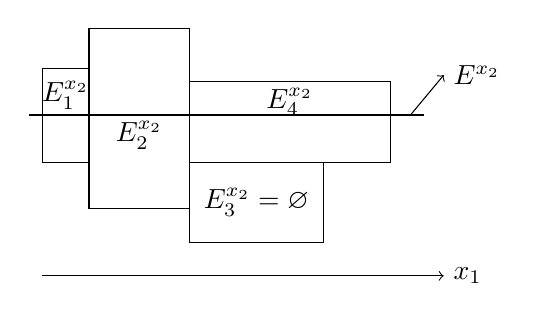
\begin{tikzpicture}[scale=0.85]
  \draw (0,1) rectangle (0.7,2.4);
  \draw (0.7,0.3) rectangle (2.2,3);
  \draw (2.2,1) rectangle (5.2,2.2);
  \draw (2.2,-0.2) rectangle (4.2,1);
  \draw[thick] (-0.2,1.7)--(5.7,1.7);
  \node at (0.35,2) {$E_1^{x_2}$};
  \node at (1.45,1.4) {$E_2^{x_2}$};
  \node at (3.7,1.9) {$E_4^{x_2}$};
  \node at (3.2,0.4) {$E_3^{x_2}=\varnothing$};
  \node[right] at (6,2.3) {$E^{x_2}$};
  \draw[->] (5.5,1.7)--(6,2.3);
  \draw[->] (0,-0.7)--(6,-0.7) node[right] {$x_1$};
\end{tikzpicture}
\end{center}
\[
\begin{aligned}
  (\mu_1\times\mu_2)(E)
  &=\sum_{j=1}^{\infty}(\mu_1\times\mu_2)(E_j)\\
  &=\sum_{j=1}^{\infty}\int_{X_2}\mu_1(E_j^{x_2})\,d\mu_2\\
  &=\int_{X_2}\sum_{j=1}^{\infty}\mu_1(E_j^{x_2})\,d\mu_2
  =\int_{X_2}\mu_1(E^{x_2})\,d\mu_2.
\end{aligned}
\]

\textbf{步骤 3.} 假使 $E\in\mathcal{A}_{\sigma\delta}$。

假如 $(\mu_1\times\mu_2)(E)<\infty$ 已经解决，那么使用 $X_1,X_2$ 的 $\sigma$-有限性，能得到一列有限测度的矩形 $F_j\times G_j\uparrow X$。考虑 $E\cap(F_j\times G_j)$ 就能解决问题。下设 $(\mu_1\times\mu_2)(E)<\infty$。

由定义，$E=\bigcap_{j=1}^{\infty}B_j$。不妨设 $B_j\downarrow E$，否则考虑 $B'_j=\bigcap_{s=1}^{j}B_s$ 即可。
\[
  E^{x_2}=\bigcap_{j=1}^{\infty}B_j^{x_2}\quad\text{可测},
\]
\[
  \mu_1(E^{x_2})=\lim_{j\to\infty}\mu_1(B_j^{x_2})\quad\text{可测}.
\]
\[
\begin{aligned}
  (\mu_1\times\mu_2)(E)
  &=\lim_{j\to\infty}(\mu_1\times\mu_2)(B_j)\\
  &=\lim_{j\to\infty}\int_{X_2}\mu_1(B_j^{x_2})\,d\mu_2\\
  &\overset{(*)}{=}\int_{X_2}\lim_{j\to\infty}\mu_1(B_j^{x_2})\,d\mu_2\\
  &=\int_{X_2}\mu_1(E^{x_2})\,d\mu_2.
\end{aligned}
\]
$(*)$ 使用的是\hyperref[thm:dominated-convergence]{控制收敛定理}：$|\mu_1(B_j^{x_2})|\leq\mu_1(B_1^{x_2})$，而
\[
  \int_{X_2}\mu_1(B_1^{x_2})\,d\mu_2=(\mu_1\times\mu_2)(B_1).
\]
不妨设 $B_1$ 测度有限（因为乘积测度是由外测度限制得到的）。
\end{proof}
\begin{proposition}
如果 $E$ 是任意可测集，则 Proposition~\ref{prop:product-slices-sigma-delta} 的结论改为：$E^{x_2}$ 几乎处处可测，且 $\mu_1(E^{x_2})$ 对几乎处处的 $x_2$ 有定义。
\end{proposition}

\begin{proof}
如果 $E$ 是零测集，则存在 $F\in\mathcal{A}_{\sigma\delta}$，$F$ 是零测集，$E\subseteq F$。由于 $F$ 是零测集，
\[
  \int_{X_2}\mu_1(F^{x_2})\,d\mu_2=0
  \quad\Longleftrightarrow\quad
  F^{x_2}\text{ 几乎处处是零测集}.
\]
又 $E^{x_2}\subseteq F^{x_2}$，所以 $E^{x_2}$ 几乎处处是零测集，从而
\[
  \int_{X_2}\mu_1(E^{x_2})\,d\mu_2=0.
\]

如果 $E$ 可测，考虑 $E\subseteq F\in\mathcal{A}_{\sigma\delta}$，$F\setminus E=Z$ 是零测集。完全同样地可得到关于 $Z$ 的截面的性质。由
\[
  E^{x_2}=F^{x_2}\setminus Z^{x_2}
\]
可得 $E^{x_2}$ 所述性质。
\end{proof}
\begin{theorem}[一般 Fubini 定理]\label{thm:fubini-general}
设 $(X_1,\mathcal{M}_1,\mu_1)$ 和 $(X_2,\mathcal{M}_2,\mu_2)$ 是完备且 $\sigma$-有限的测度空间。设 $f(x_1,x_2)$ 是乘积测度空间 $(X_1\times X_2,\mathcal{M},\mu_1\times\mu_2)$ 上的可积函数，则：
\begin{enumerate}
  \item[(1)] 对几乎处处的 $x_2\in X_2$，截面函数
  \[
    f^{x_2}(x_1)=f(x_1,x_2)
  \]
  在 $(X_1,\mu_1)$ 上可积。
  \item[(2)] 函数
  \[
    x_2\longmapsto\int_{X_1}f(x_1,x_2)\,d\mu_1
  \]
  在 $X_2$ 上可积。
  \item[(3)]
  \[
    \int_{X_2}\left(\int_{X_1}f(x_1,x_2)\,d\mu_1\right)d\mu_2
    =\int_{X_1\times X_2}f\,d(\mu_1\times\mu_2).
  \]
\end{enumerate}
\end{theorem}
\begin{proof}
这些结论在有限线性组合下保持成立，因此只需考虑非负函数。当 $f=\chi_E$ 且 $E$ 的测度有限时，结论已包含在前一个命题中。因此结论对简单函数成立，再由\hyperref[thm:monotone-convergence]{单调收敛定理}，对所有非负函数成立。将结论应用于正负部分，即得到可积函数的情形。
\end{proof}
\begin{remark}
这里的乘积测度定义在可测矩形生成的 $\sigma$-代数 $\mathcal M_1\otimes\mathcal M_2$ 上，尚未完备化。即使两个因子测度空间都完备，这个乘积空间也不一定完备。将乘积空间完备化后，上面的 Fubini 定理仍然成立。

对于 $\mathcal M_1\otimes\mathcal M_2$-可测函数，定理不需要因子空间完备，而且每个切片都可测。原书在零测集的处理步骤中使用了因子空间的完备性：零测切片的任意子集仍可测。这个条件保证完备化后的版本仍有几乎处处的切片可测性。
\end{remark}
\begin{theorem}[Tonelli 定理]\label{thm:tonelli-general}
设 $(X,\mathcal M,\mu)$、$(Y,\mathcal N,\nu)$ 都是 $\sigma$-有限测度空间，$f:X\times Y\to[0,+\infty]$ 对乘积 $\sigma$-代数可测，则
\[
\begin{aligned}
\int_{X\times Y}f\,d(\mu\times\nu)
&=\int_X\left(\int_Yf(x,y)\,d\nu(y)\right)d\mu(x)\\
&=\int_Y\left(\int_Xf(x,y)\,d\mu(x)\right)d\nu(y).
\end{aligned}
\]
允许这些积分都为 $+\infty$，不要求 $f$ 可积。若使用完备化后的乘积测度，切片的可测性一般只保证几乎处处成立。
\end{theorem}

\begin{proof}
用截断和单调收敛定理即可，但要用到两个空间的 $\sigma$-有限性。

选可测集 $A_n\uparrow X$、$B_n\uparrow Y$，使得 $\mu(A_n)<\infty$、$\nu(B_n)<\infty$。令
\[
f_n=\min(f,n)\mathbf1_{A_n\times B_n}.
\]
则 $0\leq f_n\uparrow f$，且
\[
\int f_n\,d(\mu\times\nu)\leq n\,\mu(A_n)\nu(B_n)<\infty.
\]
因此每个 $f_n$ 都可以应用有限积分情形的\hyperref[thm:fubini-general]{Fubini 定理}。再分别对乘积积分、内层积分和外层积分使用\hyperref[thm:monotone-convergence]{单调收敛定理}，就得到
\[
\int f\,d(\mu\times\nu)
=\int_X\left(\int_Y f\,d\nu\right)d\mu,
\]
允许结果为 $+\infty$。交换两个变量，同样得到另一种积分次序。
\end{proof}
\section{带符号测度}

\begin{definition}[带符号测度]
$\sigma$-代数 $\mathcal M$ 上的带符号测度 $\nu$ 满足：
\begin{enumerate}
\item[(1)] 对每个 $E\in\mathcal M$，$\nu(E)\in(-\infty,+\infty]$。
\item[(2)] 若 $\{E_j\}\subset\mathcal M$ 两两无交，则
\[
\nu\!\left(\bigcup_{j=1}^{\infty}E_j\right)=\sum_{j=1}^{\infty}\nu(E_j).
\]
\end{enumerate}
\end{definition}

\begin{remark}
为了使上式成立，右边的和必须与各项的重排无关。因此，如果并集的测度有限，则这个级数绝对收敛。
\end{remark}

\begin{example}
$f$ 可测，令 $\nu(E)=\int_E f\,d\mu$。这里要保证 $\int f^-\,d\mu<\infty$。
\end{example}

\begin{proposition}
对于带符号测度 $\nu$，存在测度 $\mu$，使得对每个 $E\in\mathcal M$ 都有 $|\nu|(E)\leq\mu(E)$。
\end{proposition}

\begin{proof}
我们定义一个 $\mathcal M$ 上的函数
\[
|\nu|(E)=\sup\sum_{j=1}^{\infty}|\nu(E_j)|,
\]
这里上确界取遍 $E$ 的所有可测的可数划分 $E=\bigcup_{j=1}^{\infty}E_j$，其中 $E_j\in\mathcal M$ 两两无交。称 $|\nu|$ 为\textbf{全变差}。注意，$|\nu|$ 是用 $\sup$ 定义的（而不是之前从预测度到外测度的 $\inf$）。

例如，直观上，设 $f:\mathbb R\to\mathbb R$ 连续，$\nu((a,b])=f(b)-f(a)$，那么 $|\nu|((a,b])$ 即 $[a,b]$ 内的绝对变化值（联想 $\int_a^b|f'|\,dx$）。

那么 $\nu\leq|\nu|$。下面证 $|\nu|$ 是测度。

只要证：对于两两无交的 $\{E_j\}\subset\mathcal M$，$E=\bigcup_{j=1}^{\infty}E_j$，有
\[
|\nu|(E)=\sum_{j=1}^{\infty}|\nu|(E_j).
\]
由定义，存在 $\{F_{j,k}\}$，使得
\[
|\nu|(E_j)\leq\sum_k|\nu(F_{j,k})|+\varepsilon_j.
\]
而 $\{F_{j,k}\}$ 覆盖 $E$，所以
\[
|\nu|(E)\geq\sum_{j,k}|\nu(F_{j,k})|
\quad\Longrightarrow\quad
|\nu|(E)\geq\sum_j|\nu|(E_j).
\]

反之，对覆盖 $E$ 的 $\{F_k\}$，令 $F_{j,k}=F_k\cap E_j$，则 $\{F_{j,k}\}_{k=1}^{\infty}$ 覆盖 $E_j$。只要证明
\[
\sum_j|\nu|(E_j)\geq\sum_k|\nu(F_k)|,\qquad(*)
\]
再对 $\{F_k\}$ 取上确界。
\[
\sum_j|\nu|(E_j)
\geq\sum_{j,k}|\nu(F_{j,k})|
=\sum_k\left(\sum_j|\nu(F_{j,k})|\right).
\]
而 $\sum_j|\nu(F_{j,k})|\geq|\nu(F_k)|$（这由 $\sum_j\nu(F_{j,k})=\nu(F_k)$ 给出），$(*)$ 得证。
\end{proof}
\begin{theorem}[带符号测度的分解]
每个带符号测度 $\nu$ 都能写成两个非负测度之差：
\[
\nu=\nu^+-\nu^-.
\]
其中 $\nu^-$ 是有限测度。
\end{theorem}

\begin{proof}
写出正部和负部（当 $|\nu|(E)<\infty$ 时）：
\[
\nu^+(E)=\frac{|\nu|(E)+\nu(E)}2,
\qquad
\nu^-(E)=\frac{|\nu|(E)-\nu(E)}2.
\]
使用上一个结论，正部和负部是非负的。
\end{proof}

\begin{proposition}[正部和负部的另一种表达]
当 $|\nu|(E)<\infty$ 时，正部和负部也可写为
\[
\nu^+(E)=\sup\{\nu(A):A\in\mathcal M,\ A\subseteq E\},
\qquad
\nu^-(E)=-\inf\{\nu(A):A\in\mathcal M,\ A\subseteq E\}.
\]
这与上面的全变差公式等价。
\end{proposition}

\begin{proof}
记 $S=\sup\{\nu(A):A\in\mathcal M,\ A\subseteq E\}$。只要证明 $|\nu|(E)=2S-\nu(E)$。

任取可测集 $A\subseteq E$，由划分 $E=A\sqcup(E\setminus A)$，
\[
\begin{aligned}
|\nu|(E)&\geq|\nu(A)|+|\nu(E\setminus A)|\\
&\geq\nu(A)-\nu(E\setminus A)
=2\nu(A)-\nu(E).
\end{aligned}
\]
对 $A$ 取上确界，得到 $|\nu|(E)\geq2S-\nu(E)$。

反之，任取可测的可数划分 $E=\bigsqcup_jE_j$，令
\[
A=\bigcup_{\nu(E_j)\geq0}E_j.
\]
因为 $\sum_j|\nu(E_j)|\leq|\nu|(E)<\infty$，可以按正负分组，于是
\[
\begin{aligned}
\sum_j|\nu(E_j)|
&=\sum_{\nu(E_j)\geq0}\nu(E_j)-\sum_{\nu(E_j)<0}\nu(E_j)\\
&=\nu(A)-\nu(E\setminus A)
=2\nu(A)-\nu(E)\\
&\leq2S-\nu(E).
\end{aligned}
\]
对所有划分取上确界，得到 $|\nu|(E)\leq2S-\nu(E)$。所以
\[
\nu^+(E)=S=\frac{|\nu|(E)+\nu(E)}2.
\]
再由 $\nu(A)=\nu(E)-\nu(E\setminus A)$，得到
\[
-\inf_{A\subseteq E,\ A\in\mathcal M}\nu(A)
=S-\nu(E)=\frac{|\nu|(E)-\nu(E)}2=\nu^-(E).
\]
\end{proof}
\begin{definition}[Mutually singular，互相奇异]
设 $\nu$ 和 $\mu$ 是 $(X,\mathcal M)$ 上的两个带符号测度。如果存在互不相交的可测集 $A,B$，使得对所有 $E\in\mathcal M$，都有
\[
\nu(E)=\nu(A\cap E),\qquad
\mu(E)=\mu(B\cap E),
\]
则称 $\nu$ 和 $\mu$ \textbf{互相奇异}，记作 $\nu\perp\mu$。
\end{definition}
\begin{remark}
对于 $X$ 上的带符号测度 $p$ 和可测集 $A$，
\[
p(E)=p(A\cap E)\quad\text{对所有 }E\in\mathcal M\text{ 成立}
\quad\Longleftrightarrow\quad
|p|(X\setminus A)=0.
\]
也就是说，$p$ 的全部质量集中在 $A$ 上，等价于 $A$ 外的全变差为零。

因此，两个带符号测度 $p,q$ 互相奇异，等价于存在两个可测集 $C,D$，使得
\[
C\cup D=X,\qquad |p|(C)=0,\qquad |q|(D)=0.
\]
这里 $C,D$ 可以相交。也可以要求它们构成 $X$ 的一个划分，即
\[
p\perp q
\quad\Longleftrightarrow\quad
\exists C\in\mathcal M,\quad |p|(C)=0,\quad |q|(X\setminus C)=0.
\]
也就是把空间分成两块，一块对 $p$ 的全变差是零测的，另一块对 $q$ 的全变差是零测的。
\end{remark}
\begin{definition}[相对于 $\mu$ 绝对连续]
设 $\nu$ 是带符号测度，$\mu$ 是同一 $\sigma$-代数 $\mathcal M$ 上的非负测度。如果对每个 $E\in\mathcal M$，都有
\[
\mu(E)=0\quad\Longrightarrow\quad\nu(E)=0,
\]
则称 $\nu$ \textbf{相对于 $\mu$ 绝对连续}，记作 $\nu\ll\mu$。
\end{definition}
\begin{proposition}
设 $\nu$ 是 $(X,\mathcal M)$ 上的带符号测度，$\mu$ 是同一可测空间上的非负测度。考虑以下两个条件：
\begin{equation*}
\mu(E)=0\ \Longrightarrow\ \nu(E)=0,
\qquad E\in\mathcal M.\tag{※}
\end{equation*}
\begin{equation*}
\forall\varepsilon>0,\ \exists\delta>0,\ \forall E\in\mathcal M,
\quad\mu(E)<\delta\ \Longrightarrow\ |\nu(E)|<\varepsilon.\tag{$\triangle$}
\end{equation*}
条件（$\triangle$）蕴含条件（※）。若 $|\nu|(X)<\infty$，则条件（※）与条件（$\triangle$）等价。
\end{proposition}
\begin{observation}
注意，可以不妨设 $\nu$ 为 $|\nu|$（这需要回忆 $|\nu|$ 的定义）。
\end{observation}
\begin{proof}
条件（$\triangle$）蕴含条件（※）是明显的。

假设 $|\nu|(X)<\infty$，且条件（※）成立。
假设对某个 $\varepsilon>0$，该命题不成立。考虑可测集合列 $\{E_n\}$，使得 $\lim_{n\to\infty}\mu(E_n)=0$，但是 $\nu(E_n)>\varepsilon$ 恒成立。

为了和条件矛盾，我们想找到一个 $\mu(E)=0$ 的集合。首先，通过把 $E_n$ 换成 $\bigcup_{k=n}^{\infty}E_k$，可以不妨设 $E_i$ 是逐渐缩小的层状集合列。取 $E=\bigcap_{i=1}^{\infty}E_i$ 就可以得到矛盾。
\end{proof}
\begin{theorem}[Lebesgue--Radon--Nikodym]\label{thm:lebesgue-radon-nikodym}
设 $\mu$ 是 $(X,\mathcal M)$ 上的 $\sigma$-有限非负测度，$\nu$ 是 $\mathcal M$ 上的 $\sigma$-有限带符号测度，即 $|\nu|$ 是 $\sigma$-有限的。则存在唯一的带符号测度 $\nu_a$ 和 $\nu_s$，使得
\[
\nu_a\ll\mu,\qquad
\nu_s\perp\mu,\qquad
\nu=\nu_a+\nu_s.
\]
这里 $\nu_a$ 和 $\nu_s$ 都定义在原来的 $\sigma$-代数 $\mathcal M$ 上。
此外，$\nu_a$ 可以写成 $d\nu_a=f\,d\mu$，即
\[
\nu_a(E)=\int_E f(x)\,d\mu(x),\qquad E\in\mathcal M,
\]
其中 $f$ 是扩展意义下的 $\mu$-可积函数，即 $\int_X f^-\,d\mu<\infty$，允许 $\int_X f^+\,d\mu=+\infty$。
\end{theorem}
\begin{proof}
略。
\end{proof}
\begin{remark}
若 $\nu\geq0$，则 $\nu_a\geq0$，$\nu_s\geq0$。
\end{remark}
\chapter{勒贝格理论}

\section{Borel 测度和 Lebesgue 测度}



\begin{definition}
定义
\[
m^*(E)=\inf\left\{\sum_{k=1}^{\infty}(b_k-a_k):
E\subset\bigcup_{k=1}^{\infty}(a_k,b_k)\right\}.
\]
令 $\mathcal{M}$ 为所有关于此外测度的 Carathéodory 可测集组成的 $\sigma$-代数。将此外测度限制到 $\mathcal{M}$ 上，得到 Lebesgue 测度，$\mathcal{M}$ 即 Lebesgue 可测集组成的集合族。
\end{definition}
\begin{definition}\label{def:lebesgue-outer-measure-rn}
在 $\mathbb{R}^n$ 中，用可数个开矩形或闭矩形覆盖，以矩形体积之和取下确界，定义 Lebesgue 外测度
\[
m^*(E)=\inf\left\{\sum_{k=1}^{\infty}|R_k|:
E\subset\bigcup_{k=1}^{\infty}R_k\right\},
\qquad
|R_k|=\prod_{i=1}^{n}(b_{k,i}-a_{k,i}).
\]
这里矩形的边平行于坐标轴，开、闭矩形覆盖得到的外测度相同。$\mathcal{M}$ 是所有 Carathéodory 可测集组成的 $\sigma$-代数，即 Lebesgue 可测集组成的集合族。将此外测度限制到 $\mathcal{M}$ 上，得到 Lebesgue 测度。
\end{definition}
以下用 $m^*$ 表示 Lebesgue 外测度，用 $m$ 表示 Lebesgue 测度；对可测集 $E$，有 $m(E)=m^*(E)$。




\begin{remark}
一般我们需要一个代数 $\mathcal{A}$ 上的预测度，才能给出一个 $2^X$ 上的外测度。
但是这里直接用 $(a_k,b_k)$ 的并定义，实际上也能得到外测度。
具体地，读者可以想见：对于任意子集族 $\mathcal{P}\subset 2^X$，只要指定
$f:\mathcal{P}\to[0,+\infty)$，便都能用
\[
\inf\left\{\sum_{i=1}^{\infty}f(P_i):
P_i\in\mathcal{P},\ E\subset\bigcup_{i=1}^{\infty}P_i\right\}
\]
给出外测度。实际上，之后的 Hausdorff 测度也会类似给出。
\end{remark}

\begin{proposition}\label{prop:interval-lebesgue-measure}
对于 $a\leq b$，有
\[
m^*([a,b])=b-a.
\]
此外，区间都是 Lebesgue 可测的。
\end{proposition}
\begin{proof}
使用开区间覆盖定义的版本，这样能使用紧性定理化归为有限个开区间的情形。然后的处理是初等的。开区间 $(a,b)$ 的外测度可类似处理。
下面证明 $[a,b]$ 的可测性。任取 $X\subset\mathbb{R}$，令
\[
P=X\cap[a,b],\qquad Q=X\cap(\mathbb{R}\setminus[a,b]),
\]
则 $X=P\cup Q$。只要证明
\[
m^*(P\cup Q)\geq m^*(P)+m^*(Q).
\]
任取 $P\cup Q$ 的闭区间覆盖 $\{[a_k,b_k]\}_{k=1}^{\infty}$，将每个覆盖区间在 $a,b$ 处分割，得到分别覆盖 $P,Q$ 的区间族，记为 $\{I_j\}$ 和 $\{J_\ell\}$。分割不改变总长度，因此
\[
\sum_{k=1}^{\infty}(b_k-a_k)
=\sum_j|I_j|+\sum_\ell|J_\ell|
\geq m^*(P)+m^*(Q).
\]
由覆盖的任意性，取下确界即得所需不等式，故 $[a,b]$ 可测。
\end{proof}

\begin{remark}
注意，假如用闭区间覆盖定义，就要多绕一步。
\end{remark}

\begin{proposition}[平移不变性]
外测度与测度在平移下不变，且平移保持可测性。具体地，对于 $E\subset\mathbb{R}^d$ 和 $h\in\mathbb{R}^d$，有
\[
m^*(E+h)=m^*(E).
\]
若 $E$ 可测，则 $E+h$ 可测，且 $m(E+h)=m(E)$。
\end{proposition}

\begin{proposition}[伸缩性质]
正伸缩保持可测性。对于可测集 $E\subset\mathbb{R}^d$ 和 $\delta>0$，$\delta E$ 可测，且
\[
m(\delta E)=\delta^d m(E).
\]
\end{proposition}

\begin{proposition}[反射不变性]
对于 $E\subset\mathbb{R}^d$，$E$ 可测当且仅当 $-E$ 可测，且可测时有
\[
m(-E)=m(E).
\]
\end{proposition}
\begin{proposition}\label{prop:lebesgue-complete}
Lebesgue 测度是完备的。因此，在 Lebesgue 测度空间中，若 $f$ 可测，且 $g=f$ 几乎处处成立，则 $g$ 可测。
\end{proposition}
\begin{theorem}[Lebesgue 可测集的乘积]
设 $E_1\subseteq\mathbb R^{d_1}$、$E_2\subseteq\mathbb R^{d_2}$ 都是 Lebesgue 可测集。则 $E_1\times E_2$ 是 $\mathbb R^{d_1+d_2}$ 中的 Lebesgue 可测集，且
\[
m_{d_1+d_2}(E_1\times E_2)=m_{d_1}(E_1)m_{d_2}(E_2).
\]
其中约定 $0\cdot\infty=0$。
\end{theorem}
\begin{proof}
只需证 $E=E_1\times E_2$ 可测，再使用之前的\hyperref[thm:tonelli-general]{Tonelli 定理}计算 $E_1\times E_2$ 的测度即可。

想法是：假如我们能用好的集合 $G_1,G_2$ 逼近 $E_j$，而且 $G_1\times G_2$ 性质也好，使得 $m((G_1\times G_2)\triangle(E_1\times E_2))=0$，则由 Lebesgue 测度的完备性（Proposition~\ref{prop:lebesgue-complete}），即可从 $G_1\times G_2$ 可测推出 $E$ 可测。

Theorem~\ref{thm:lebesgue-gdelta-fsigma} 中叙述的 $G_\delta$ 集或 $F_\sigma$ 集就是所谓的好的集合。
\end{proof}

\begin{definition}[Borel 集与 Borel 测度]
$\mathbb{R}^n$ 中由所有开集生成的 $\sigma$-代数称为 \textbf{Borel $\sigma$-代数}，记为 $\mathcal{B}_{\mathbb{R}^n}$。它的元素称为 \textbf{Borel 集}。
定义在 Borel $\sigma$-代数上的测度称为 \textbf{Borel 测度}。
\end{definition}
\begin{proposition}
对于正整数 $d_1,d_2$，有
\[
\mathcal{B}_{\mathbb{R}^{d_1}}\otimes\mathcal{B}_{\mathbb{R}^{d_2}}
=\mathcal{B}_{\mathbb{R}^{d_1+d_2}}.
\]
\end{proposition}
\begin{center}
\setlength{\fboxsep}{12pt}
\fcolorbox{red}{red!8}{\parbox{0.85\textwidth}{\centering\Large\bfseries\color{red}Borel 张量积等式的说明尚未写完，待补充。}}
\end{center}
\begin{example}
Lebesgue 测度在 $\mathcal{B}_{\mathbb{R}^n}$ 上的限制是一个 Borel 测度。
\end{example}
\begin{remark}
在乘积 $\sigma$-代数上定义的 Lebesgue 测度的乘积，不是完整的高维 Lebesgue 测度；其完备化才是高维 Lebesgue 测度。
\end{remark}

\noindent
下面引出一个 Borel 不可测但是 Lebesgue 可测的例子。
\begin{definition}[Cantor 集]
令 $E_0=[0,1]$，每一步从 $E_{i-1}$ 的每个闭区间中删去中间三分之一的开区间，得到 $E_i$。称
\[
C=\bigcap_{i=0}^{\infty}E_i
\]
为 \textbf{Cantor 集}。
\end{definition}

\begin{remark}
Cantor 集恰好由存在一个仅含数字 $0,2$ 的三进制展开的数构成，即
\[
C=\left\{\sum_{k=1}^{\infty}\frac{a_k}{3^k}:a_k\in\{0,2\}\right\}.
\]
\end{remark}
\begin{proposition}
$\mathbb{R}$ 上的 Borel 集的个数与 $\mathbb{R}$ 等势。
\end{proposition}
\begin{proof}
略。
\end{proof}

\begin{proposition}
Cantor 集不可数。
\end{proposition}
\begin{proof}
由上述 remark，可以构造从 Cantor 集到 $[0,1]$ 的满射：
\[
\sum_{k=1}^{\infty}\frac{a_k}{3^k}
\longmapsto
\sum_{k=1}^{\infty}\frac{a_k/2}{2^k},
\qquad a_k\in\{0,2\}.
\]
因此 Cantor 集不可数。又因为 $C\subset[0,1]$，故 $|C|=\mathfrak{c}$，其中 $\mathfrak{c}=|\mathbb{R}|$。
\end{proof}

\begin{theorem}
存在一个 Cantor 集的子集是 Lebesgue 可测的，但不是 Borel 集。
\end{theorem}
\begin{proof}
考虑 Cantor 集的所有子集，其个数为 $2^{\mathfrak{c}}>\mathfrak{c}$，而 $\mathbb{R}$ 上的 Borel 集只有 $\mathfrak{c}$ 个，因此存在 $E\subset C$ 不是 Borel 集。
另一方面，$C\subset E_i$，且 $m(E_i)=(2/3)^i$，故 $m(C)=0$。由 Lebesgue 测度的完备性，$C$ 的所有子集都是 Lebesgue 可测的，且测度为零。因此这样的 $E$ 即为所需例子。
\end{proof}
\noindent
下面介绍 $\mathbb{R}$ 上的 Borel 测度和单调函数的关系。
\begin{definition}[增函数的正规化]
设 $F:\mathbb{R}\to\mathbb{R}$ 为非减函数。令
\[
\widetilde F(x)=F(x^+)=\lim_{t\downarrow x}F(t),
\]
称为 $F$ 的\textbf{正规化}。正规化后的函数非减且右连续；非减且右连续的函数称为\textbf{正规的增函数}。
\end{definition}

\begin{theorem}
设 $F$ 是 $\mathbb{R}$ 上正规的增函数，则在 $\mathbb{R}$ 的 Borel 集上存在唯一的测度 $\mu$，也记为 $dF$，使得
\[
\mu((a,b])=F(b)-F(a),\qquad a<b.
\]
反之，若 $\mu$ 是 Borel 集上的测度，且在有界区间上有限，则函数
\[
F(x)=
\begin{cases}
\mu((0,x]),&x>0,\\
0,&x=0,\\
-\mu((x,0]),&x<0
\end{cases}
\]
是正规的增函数。
\end{theorem}
\begin{proof}
对“反之”部分，直接验证即可。

对正向部分，在 $\mathbb{R}$ 的所有子集上定义函数
\[
\mu_*(E)=\inf\left\{\sum_{j=1}^{\infty}\bigl(F(b_j)-F(a_j)\bigr):
E\subset\bigcup_{j=1}^{\infty}(a_j,b_j]\right\}.
\]
这里下确界取遍 $E$ 的所有形如 $\bigcup_{j=1}^{\infty}(a_j,b_j]$ 的覆盖。（回忆 Definition~\ref{def:lebesgue-outer-measure-rn} 后面的 remark。）
进一步，
\[
\mu_*((a,b])=F(b)-F(a),\qquad\text{而且 }(a,b]\text{ 都是 Carathéodory 可测的。}
\]
这里的论证和 Proposition~\ref{prop:interval-lebesgue-measure} 几乎相同。
这样，$\mu_*$ 可以限制在所有 Borel 集上作为测度。
\end{proof}
\begin{theorem}[多维 Lebesgue--Stieltjes 测度]\label{thm:multidimensional-stieltjes}
设 $F:\mathbb{R}^n\to\mathbb{R}$ 为有限值函数。对于有界半开矩形
\[
(a,b]:=\prod_{i=1}^n(a_i,b_i],\qquad a_i<b_i,
\]
以及 $\varepsilon=(\varepsilon_1,\ldots,\varepsilon_n)\in\{0,1\}^n$，记
\[
c_{\varepsilon,i}=
\begin{cases}
a_i,&\varepsilon_i=0,\\
b_i,&\varepsilon_i=1,
\end{cases}
\qquad |\varepsilon|=\sum_{i=1}^n\varepsilon_i.
\]
定义 $F$ 在矩形 $(a,b]$ 上的\textbf{混合增量}为
\[
\Delta_{a,b}F
=\sum_{\varepsilon\in\{0,1\}^n}
(-1)^{n-|\varepsilon|}F(c_{\varepsilon,1},\ldots,c_{\varepsilon,n}).
\]
假设 $F$ 满足以下两个条件：
\begin{enumerate}
\item[(1)] 对每个有界半开矩形 $(a,b]$，都有
\[
\Delta_{a,b}F\geq0.
\]
这个条件称为 $F$ 是\textbf{$n$ 维递增的}。特别地，二维时要求对所有 $a_1<b_1$、$a_2<b_2$，都有
\[
F(b_1,b_2)-F(a_1,b_2)-F(b_1,a_2)+F(a_1,a_2)\geq0.
\]
\item[(2)] $F$ 从右上方连续：若对每个 $i$ 都有 $x_i^{(k)}\downarrow x_i$，则
\[
F(x_1^{(k)},\ldots,x_n^{(k)})\longrightarrow F(x_1,\ldots,x_n).
\]
这里允许某些坐标保持不变。
\end{enumerate}
则在 $\mathbb{R}^n$ 的 Borel 集上存在唯一的测度 $\mu$，也记为 $dF$，在有界矩形上有限，且满足
\[
\boxed{\mu((a,b])=\Delta_{a,b}F.}
\]
反之，若 $\mu$ 是 $\mathbb{R}^n$ 的 Borel 集上的测度，且在有界矩形上有限，记
\[
I(t)=
\begin{cases}
(0,t],&t>0,\\
\varnothing,&t=0,\\
(t,0],&t<0.
\end{cases}
\]
定义归一化后的函数
\[
F(x_1,\ldots,x_n)=
\begin{cases}
(-1)^{\#\{i:x_i<0\}}\displaystyle\mu\!\left(\prod_{i=1}^n I(x_i)\right),
&\text{所有 }x_i\ne0,\\[4pt]
0,&\text{至少一个 }x_i=0.
\end{cases}
\]
则 $F$ 满足上述两个条件，并且对每个有界半开矩形都有
\[
\Delta_{a,b}F=\mu((a,b]).
\]

\end{theorem}

\begin{remark}[归一化后的函数一般不对坐标递增]
上述归一化后的 $F$ 一般不对每个坐标分别递增。例如，二维 Lebesgue 测度对应的函数是 $F(x,y)=xy$。当 $y<0$ 时，$F(x,y)$ 随 $x$ 增大而减小，但 $\Delta_{a,b}F=(b_1-a_1)(b_2-a_2)>0$。

另一方面，仅要求对每个坐标分别递增也不够。例如 $F(x,y)=-e^{-x-y}$ 对两个坐标都严格递增，但在 $(0,1]\times(0,1]$ 上，$F(1,1)-F(0,1)-F(1,0)+F(0,0)=-(1-e^{-1})^2<0$。

因此，高维条件是每个矩形上的混合增量非负，而不是对每个坐标分别递增。
\end{remark}

\begin{remark}[测度的唯一性与函数的唯一性]
给定满足定理条件的 $F$，由 $\mu((a,b])=\Delta_{a,b}F$ 确定的 Borel 测度 $\mu$ 唯一；但给定 $\mu$，若不作归一化，对应的 $F$ 不唯一。

一维中，给 $F$ 加上常数不会改变测度。二维中，
\[
\widetilde F(x,y)=F(x,y)+g(x)+h(y)
\]
也不会改变任何矩形增量。若还要求 $\widetilde F$ 满足定理中的连续性条件，可取右连续的 $g,h$。一般地，加入任何不依赖至少一个坐标的项，其完整的 $n$ 重混合增量都为零，因而不改变测度。

如果要求
\[
F(x_1,\ldots,x_n)=0\qquad\text{只要至少一个 }x_i=0,
\]
则由 $\mu$ 确定的 $F$ 唯一，正是定理反向部分给出的带符号矩形测度公式。
\end{remark}
\begin{center}
\setlength{\fboxsep}{12pt}
\fcolorbox{red}{red!8}{\parbox{0.85\textwidth}{\centering\Large\bfseries\color{red}第 2.1 节尚未写完，待补充。}}
\end{center}
\section{Lebesgue 测度和积分的特殊性质}

\begin{proposition}[开集外逼近与闭集内逼近]\label{prop:lebesgue-open-closed-approx}
设 $E\subseteq\mathbb R^n$ 是 Lebesgue 可测集。则对任意 $\varepsilon>0$：
\begin{enumerate}
\item[(1)] 存在开集 $O\supseteq E$，使得 $m(O\setminus E)<\varepsilon$。
\item[(2)] 存在闭集 $F\subseteq E$，使得 $m(E\setminus F)<\varepsilon$。
\end{enumerate}
\end{proposition}

\begin{proof}
第一项就是可测性的定义。对于第二项，对可测集 $E^c$ 使用第一项，取开集 $O\supseteq E^c$，使得 $m(O\setminus E^c)<\varepsilon$。令 $F=O^c$，则 $F$ 是闭集，$F\subseteq E$，且 $E\setminus F=O\setminus E^c$，所以 $m(E\setminus F)<\varepsilon$。
\end{proof}
\begin{remark}[有限测度集合的紧集内逼近]\label{rem:lebesgue-compact-inner-approx}
若 $E\subseteq\mathbb R^n$ 可测且 $m(E)<\infty$，则对任意 $\varepsilon>0$，存在紧集 $K\subseteq E$，使得 $m(E\setminus K)<\varepsilon$。

取闭集 $F\subseteq E$，使得 $m(E\setminus F)<\varepsilon/2$。令 $B_j=\{x\in\mathbb R^n:|x|\leq j\}$，则 $K_j=F\cap B_j$ 是紧集，且 $E\setminus K_j\downarrow E\setminus F$。由 $m(E)<\infty$，有 $m(E\setminus K_j)\to m(E\setminus F)<\varepsilon/2$，所以取充分大的 $j$ 即可。
\end{remark}

\begin{definition}
$G_\delta$ 集是可数个开集的交，$F_\sigma$ 集是可数个闭集的并。
\end{definition}

\begin{theorem}\label{thm:lebesgue-gdelta-fsigma}
对于 Lebesgue 可测集 $E\subseteq\mathbb R^n$，存在 $G_\delta$ 集 $G$ 作外逼近，$F_\sigma$ 集 $F$ 作内逼近，使得
\[
E\subseteq G,\qquad m(G\setminus E)=0,
\]
\[
F\subseteq E,\qquad m(E\setminus F)=0.
\]
\end{theorem}

\begin{proof}
使用 Proposition~\ref{prop:lebesgue-open-closed-approx}，并使用 $F_\sigma$、$G_\delta$ 的定义（对一列误差 $\varepsilon_k\to0$ 的集合取可数交、并）。
\end{proof}
\begin{proposition}[有限矩形逼近]\label{prop:finite-rectangle-approx}\label{prop:closed-egorov}
设 $E\subseteq\mathbb R^n$ 是 Lebesgue 可测集，且 $m(E)<\infty$。则对任意 $\varepsilon>0$，存在有限个开球的并 $U$，使得 $m(E\triangle U)<\varepsilon$；也存在有限个闭矩形 $R_1,\ldots,R_N$，令 $F=\bigcup_{j=1}^N R_j$，使得
\[
m(E\triangle F)<\varepsilon.
\]
这里 $E\triangle F=(E\setminus F)\cup(F\setminus E)$ 是对称差，闭矩形可以取为闭立方体。
\end{proposition}

\begin{proof}
先证明有限球并逼近。由紧集内逼近和开集外逼近，选取紧集 $K$ 和开集 $O$，使得
\[
K\subseteq E\subseteq O,\qquad
m(E\setminus K)<\varepsilon/2,\qquad
m(O\setminus E)<\varepsilon/2.
\]
用包含于 $O$ 的开球覆盖紧集 $K$，取有限子覆盖，其并 $U$ 满足 $K\subseteq U\subseteq O$。于是
\[
m(E\triangle U)\leq m(E\setminus K)+m(O\setminus E)<\varepsilon.
\]

再证明有限矩形并逼近。先取有限球并 $U$，使得 $m(E\triangle U)<\varepsilon/2$。每个球都能用有限个闭矩形的并在对称差测度上任意小地逼近，所以可取有限闭矩形并 $F$，使得 $m(U\triangle F)<\varepsilon/2$。于是
\[
m(E\triangle F)\leq m(E\triangle U)+m(U\triangle F)<\varepsilon.
\]
\end{proof}
\begin{remark}
必要时可以不妨设矩形 $R_1,\ldots,R_N$ 两两不交。
\end{remark}
\begin{proposition}[Egorov 定理的闭集版本]
设 $E\subseteq\mathbb R^n$ 可测且 $m(E)<\infty$，$\{f_k\}$ 是 $E$ 上的一列可测函数，且 $f_k\to f$ 几乎处处成立。则对任意 $\varepsilon>0$，存在闭集 $F\subseteq E$，使得 $m(E\setminus F)<\varepsilon$，且 $f_k$ 在 $F$ 上一致收敛到 $f$。
\end{proposition}

\begin{proof}
由一般测度空间上的\hyperref[thm:egorov-general]{Egorov 定理}，取可测集 $A\subseteq E$，使得 $m(E\setminus A)<\varepsilon/2$，且 $f_k$ 在 $A$ 上一致收敛。

再使用 Proposition~\ref{prop:lebesgue-open-closed-approx} 的\textbf{闭集内逼近}，取闭集 $F\subseteq A$，使得 $m(A\setminus F)<\varepsilon/2$。于是 $m(E\setminus F)<\varepsilon$，且一致收敛在子集 $F$ 上仍然成立。
\end{proof}
\begin{theorem}[Lusin 定理]
设 $E\subseteq\mathbb R^n$ 是 Lebesgue 可测集，$m(E)<\infty$，$f:E\to\mathbb R$ 是有界可测函数。则对任意 $\varepsilon>0$，存在闭集 $F\subseteq E$，使得
\[
m(E\setminus F)<\varepsilon,
\]
且 $f|_F$ 连续。
\end{theorem}
\begin{proof}[Proof 1]\phantomsection\label{proof:lusin-one}
\textbf{想法：使用一致收敛性来保证 $f$ 的连续性。}先让简单函数在一个大闭集上的限制连续，再利用连续函数的一致极限仍连续。

由有界可测函数的简单函数逼近，取
\[
s_k=\sum_{j=1}^{N_k}a_{k,j}\mathbf1_{A_{k,j}},
\]
其中对每个 $k$，$A_{k,j}$ 两两无交，并为 $E$，且 $s_k\to f$ 一致收敛。

使用 Proposition~\ref{prop:lebesgue-open-closed-approx} 的闭集内逼近，对每个 $A_{k,j}$ 选取闭集 $F_{k,j}\subseteq A_{k,j}$，使得
\[
m(A_{k,j}\setminus F_{k,j})<\frac{\varepsilon}{2^{k+1}N_k}.
\]
令 $F_k=\bigcup_{j=1}^{N_k}F_{k,j}$，则 $F_k$ 闭，且 $m(E\setminus F_k)<\varepsilon/2^{k+1}$。

在 $F_k$ 中，每个 $F_{k,j}$ 既是相对闭集，也是相对开集，因为其补集是其余有限个闭集的并。$s_k$ 在每个 $F_{k,j}$ 上为常数，所以 $s_k|_{F_k}$ 连续。

最后取 $F=\bigcap_{k=1}^{\infty}F_k$，则 $F$ 闭，$F\subseteq E$，且
\[
m(E\setminus F)\leq\sum_{k=1}^{\infty}m(E\setminus F_k)<\varepsilon.
\]
每个 $s_k|_F$ 都连续，又因为 $s_k|_F\to f|_F$ 一致收敛，所以 $f|_F$ 连续。
\end{proof}
\begin{proof}[Proof 2]\phantomsection\label{proof:lusin-two}
仍然需要简单函数的逼近，记为 $(*)$。

\begin{lemma}
对于 Lebesgue 可测函数 $f$，存在一列阶梯函数 $\{\varphi_k\}$，使得 $\varphi_k\to f$ 几乎处处。这里阶梯函数指的是 $\sum_{k=1}^N a_k\mathbf1_{R_k}$，$R_k$ 是闭矩形。
\end{lemma}

\begin{observation}
由 $(*)$，只要对 $\mathbf1_E$ 进行逼近。
\end{observation}

\textbf{引理的证明.} 由 Proposition~\ref{prop:finite-rectangle-approx}，对 $n\in\mathbb Z_{>0}$，取两两无交的闭矩形 $Q_{n,1},\ldots,Q_{n,N_n}$，使得
\[
m\!\left(\left(\bigcup_iQ_{n,i}\right)\triangle E\right)<\varepsilon_n.
\]
现在 $\varphi_n=\sum_i\mathbf1_{Q_{n,i}}$，在除了一个测度小于 $\varepsilon_n$ 的集合之外等于 $f=\mathbf1_E$。记
\[
E_n=\{x:\varphi_n(x)\ne f(x)\},\qquad m(E_n)<\varepsilon_n.
\]
令 $\varepsilon_n=2^{-n}$，$F_k=\bigcup_{n\geq k+1}E_n$，则
\[
m(F_k)\leq\sum_{n\geq k+1}\varepsilon_n=2^{-k}.
\]
从而 $F=\bigcap_kF_k$ 是零测集，而且 $\varphi_k\to f$ 在 $\mathbb R^n\setminus F$ 上成立。

（注意：这并非简单；一开始我们把 $E_n$ 转化为 $F_k$，从而
\[
\bigcap_kF_k
=\{x:\forall k,\ \exists n\geq k+1,\ \varphi_n(x)\ne\mathbf1_E(x)\}
=\{x:\text{存在一列 }\{k_n\},\ \varphi_{k_n}(x)\ne\mathbf1_E(x)\text{ 恒成立}\},
\]
即不收敛点。一开始想加条件 $\bigcup_iQ_{n,i}\subseteq\bigcup_jQ_{n+1,j}$，但是有困难（我认为）。）

回到原题。取阶梯函数 $f_k\to f$ 几乎处处。存在集合 $D_k$，使得 $m(D_k)<2^{-k}$，且 $f_k$ 在 $D_k$ 外连续。

由\hyperref[thm:egorov-general]{Egorov 定理}，取可测集 $A\subseteq E$，使得 $m(E\setminus A)<\varepsilon/3$，且 $f_k$ 在 $A$ 上一致收敛。选 $N$，使得 $\sum_{k\geq N}2^{-k}<\varepsilon/3$，令
\[
F'=A\setminus\bigcup_{k\geq N}D_k.
\]
则每个 $k\geq N$ 的 $f_k|_{F'}$ 都连续，且一致收敛到 $f|_{F'}$，所以 $f|_{F'}$ 连续。

最后由闭集内逼近，取闭集 $F\subseteq F'$，使得 $m(F'\setminus F)<\varepsilon/3$。于是 $m(E\setminus F)<\varepsilon$，且 $f|_F$ 连续。
\end{proof}
\begin{remark}
注意，实际上 \hyperref[proof:lusin-one]{Proof 1} 和 \hyperref[proof:lusin-two]{Proof 2} 本身没有什么区别，因为可以看到 \hyperref[proof:lusin-one]{Proof 1} 中用到的 Proposition~\ref{prop:closed-egorov} 也是用 \hyperref[proof:lusin-two]{Proof 2} 中用到的 Proposition~\ref{prop:finite-rectangle-approx} 来证明的。
\end{remark}
\begin{remark}
也可以不要求 $f$ 有界，允许 $f:E\to[-\infty,+\infty]$ 为可测函数。此时，对任意 $\varepsilon>0$，仍存在闭集 $F\subseteq E$，使得 $m(E\setminus F)<\varepsilon$，且 $f|_F$ 连续；这里的连续性是指取值于扩展实数 $[-\infty,+\infty]$（赋予序拓扑）的连续性。
\end{remark}
\begin{lemma}[阶梯函数的 $L^1$ 逼近]\label{lem:step-functions-l1-density}
若 $f\in L^1(\mathbb R^d)$，则存在一列阶梯函数 $\{\varphi_n\}$，使得 $\|f-\varphi_n\|_1\to0$。这里阶梯函数是有限个有界闭矩形的示性函数的线性组合。
\end{lemma}

\begin{proof}
给定 $\varepsilon>0$，由\hyperref[thm:simple-functions-lp-density]{简单函数的稠密性}，先取简单函数 $s=\sum_{j=1}^N a_j\mathbf1_{E_j}$，其中 $m(E_j)<\infty$，使得 $\|f-s\|_1<\varepsilon/2$。再由 Proposition~\ref{prop:finite-rectangle-approx}，取有限闭矩形并 $A_j$ 逼近各个 $E_j$，使得 $\sum_{j=1}^N|a_j|\,m(E_j\triangle A_j)<\varepsilon/2$。

令阶梯函数 $\varphi=\sum_{j=1}^N a_j\mathbf1_{A_j}$，则
\[
\|f-\varphi\|_1
\leq\|f-s\|_1+\|s-\varphi\|_1
\leq\|f-s\|_1+\sum_{j=1}^N|a_j|\,m(E_j\triangle A_j)
<\varepsilon.
\]
取 $\varepsilon=1/n$，即得所需的阶梯函数列。
\end{proof}
\begin{theorem}[总结]
\textbf{Littlewood 的三个原则。}
\begin{enumerate}
\item 可测集几乎是有限区间或矩形并。
\item 可测函数几乎连续。
\item 点态收敛几乎一致。
\end{enumerate}
Littlewood 在 1944 年由牛津大学出版社出版的《函数论讲义》第 26 页表述了这三个原则，用来概括测度论中的基本思想。
\end{theorem}
\noindent 下面介绍 Riemann 积分和勒贝格积分的关系。
\begin{theorem}
设 $f$ 在闭区间 $[a,b]$ 上 Riemann 可积。则 $f$ 可测，且
\[
\int_{[a,b]}^{R}f(x)\,dx
=\int_{[a,b]}^{L}f(x)\,dx,
\]
其中左边是通常的 Riemann 积分，右边是 Lebesgue 积分。
\end{theorem}
\begin{proof}
由 Riemann 可积性，$f$ 有界。由 Lebesgue 判据，$f$ 的不连续点集 $D$ 是零测集。$f$ 在 $[a,b]\setminus D$ 上的限制连续，因而在这个可测子集上可测；而 $D$ 的任意子集都 Lebesgue 可测，所以 $f$ 在 $[a,b]$ 上可测。又因 $f$ 有界，故 $f$ Lebesgue 可积。

由 Riemann 可积性，可取上下阶梯函数 $\varphi_k\leq f\leq\psi_k$，使得
\[
\int_a^b\varphi_k(x)\,dx\longrightarrow\int_a^b{}^{R}f(x)\,dx,
\qquad
\int_a^b\psi_k(x)\,dx\longrightarrow\int_a^b{}^{R}f(x)\,dx.
\]
阶梯函数的 Riemann 积分与 Lebesgue 积分相同。由积分的单调性，
\[
\int_a^b\varphi_k(x)\,dx
\leq\int_{[a,b]}^{L}f(x)\,dx
\leq\int_a^b\psi_k(x)\,dx.
\]
令 $k\to\infty$，由夹逼得到两个积分相同。
\end{proof}
\begin{remark}
注意，一维反常积分可能与 Lebesgue 积分不同，这与绝对可积性有关。仅反常积分存在还不够：条件收敛时，Lebesgue 积分可能没有定义。但若反常积分绝对收敛，则它与 Lebesgue 积分相同。
\end{remark}


\begin{theorem}[差变量函数的联合可测性]
设 $f:\mathbb R^d\to\mathbb R$ 是 Lebesgue 可测函数，则
\[
\widetilde f(x,y)=f(x-y)
\]
在 $\mathbb R^d\times\mathbb R^d$ 上 Lebesgue 可测。
\end{theorem}
\begin{observation}
令 $E=\{z\in\mathbb R^d:f(z)<a\}$。只要证明：$E$ 可测，则 $\widetilde E=\{(x,y):x-y\in E\}$ 在 $\mathbb R^d\times\mathbb R^d$ 中可测。
\end{observation}

\begin{lemma}\label{lem:difference-null-preimage}
\noindent 若 $A\subseteq\mathbb R^d$ 是零测集，则 $\widetilde A=\{(x,y):x-y\in A\}$ 是 $\mathbb R^{2d}$ 中的零测集。
\end{lemma}

\begin{proof}
取开集 $O\supseteq A$，使得 $m(O)$ 任意小。$\widetilde O$ 是开集，所以可以使用\hyperref[thm:tonelli-general]{Tonelli 定理}。令 $B_k=\{y:|y|\leq k\}$，由平移不变性，
\[
m\bigl(\widetilde O\cap(\mathbb R^d\times B_k)\bigr)
=\int_{B_k}m(O+y)\,dy=m(O)m(B_k).
\]
因此 $m^*(\widetilde A\cap(\mathbb R^d\times B_k))=0$。再取可数并，得到 $m^*(\widetilde A)=0$，由 Lebesgue 测度的完备性即得结论。
\end{proof}

\begin{proof}
由 Theorem~\ref{thm:lebesgue-gdelta-fsigma}，取 $G_\delta$ 集 $G\supseteq E$，使得 $m(G\setminus E)=0$。对 $G\setminus E$ 使用 Lemma~\ref{lem:difference-null-preimage}，得到 $\widetilde{G\setminus E}$ 是零测集。下面证 $\widetilde G$ 可测。

写 $G=\bigcap_{i=1}^{\infty}G_i$，其中 $G_i$ 是开集，则
\[
\widetilde G=\{(x,y):x-y\in G_i,\ i\geq1\}
=\bigcap_{i=1}^{\infty}\widetilde G_i.
\]
现在只要对开集证明原定理即可。对于开集 $P$，$\{(x,y):x-y\in P\}$ 也是开集，所以 $\widetilde G$ 可测。再由 $\widetilde E=\widetilde G\setminus\widetilde{G\setminus E}$，得到 $\widetilde E$ 可测，得证。
\end{proof}

\begin{remark}
注意，每个切片都可测，不一定能推出原集合可测，即使是在乘积测度完备化的意义下。
\end{remark}
\begin{remark}
这个证明用到了乘积空间 $\mathbb R^d\times\mathbb R^d$ 上 Lebesgue 测度的完备性。
\end{remark}
\section{实函数的微分}

\begin{definition}[极大函数]
设 $f\in L^1(\mathbb R^d)$，定义其极大函数
\[
f^*(x)=\sup_{x\in B}\frac{1}{m(B)}\int_B|f(y)|\,dy,
\]
其中 $B$ 取遍包含 $x$ 的开球。
\end{definition}

\begin{proposition}\label{prop:maximal-function-weak-estimate}
设 $f\in L^1(\mathbb R^d)$，则：
\begin{enumerate}
\item[(1)] $f^*$ 可测。
\item[(2)] $f^*(x)<\infty$ 几乎处处成立。
\item[(3)] 对所有 $\alpha>0$，有
\[
m\bigl(\{x:f^*(x)>\alpha\}\bigr)\leq\frac{3^d}{\alpha}\|f\|_1.
\]
\end{enumerate}
\end{proposition}

\begin{remark}
(3) 说明 $f^*$ 可能大于 $f$，但是从整体上不会大太多。另一个直接的估计是 Chebyshev 不等式：$m(\{x:|g(x)|>\alpha\})\leq\alpha^{-1}\|g\|_1$，所以常数 $3^d$ 重要。
\end{remark}

\begin{lemma}[Vitali 覆盖引理]\label{lem:vitali-finite-balls}
设 $\mathcal B=\{B_1,\ldots,B_N\}$ 是有限个开球。则存在两两不交的 $B_{i_1},\ldots,B_{i_k}\in\mathcal B$，使得
\[
m\left(\bigcup_{i=1}^N B_i\right)\leq3^d\sum_{j=1}^k m(B_{i_j}).
\]
\end{lemma}

\begin{proof}
每次选取剩余球中半径最大的一个，并删去所有与它相交的球，直到没有球剩下。选出的球两两不交；每个被删去的球都与某个选出的球相交，且半径不大于它，所以包含在该球的三倍同心球中。因此 $\bigcup_{i=1}^N B_i\subseteq\bigcup_{j=1}^k3B_{i_j}$，取测度即得结论。
\end{proof}

\begin{proof}[Proposition~\ref{prop:maximal-function-weak-estimate} 的证明]
(1) 令 $E_\alpha=\{x:f^*(x)>\alpha\}$。对每个 $x\in E_\alpha$，存在包含 $x$ 的开球 $B_x$，使得 $m(B_x)^{-1}\int_{B_x}|f(y)|\,dy>\alpha$。同一个球对其中每个点都满足这个条件，所以 $B_x\subseteq E_\alpha$，从而 $E_\alpha$ 是开集，$f^*$ 可测。

下面证明 (3)，再结合 $\{x:f^*(x)=\infty\}=\bigcap_{n=1}^{\infty}\{x:f^*(x)>n\}$ 即得 (2)。

对 $x\in E_\alpha$ 取上述开球 $B_x$，则
\[
m(B_x)<\frac1\alpha\int_{B_x}|f(y)|\,dy.
\]
对任意紧集 $K\subseteq E_\alpha$，由紧性可取有限个球 $B_{x_1},\ldots,B_{x_N}$ 覆盖 $K$。由 Lemma~\ref{lem:vitali-finite-balls}，可选出其中两两不交的 $B_{x_{i_1}},\ldots,B_{x_{i_k}}$，使得
\[
\begin{aligned}
m(K)&\leq m\left(\bigcup_{i=1}^N B_{x_i}\right)
\leq3^d\sum_{j=1}^k m(B_{x_{i_j}})\\
&\leq\frac{3^d}{\alpha}\sum_{j=1}^k\int_{B_{x_{i_j}}}|f(y)|\,dy
\leq\frac{3^d}{\alpha}\int_{\mathbb R^d}|f(y)|\,dy.
\end{aligned}
\]
由\hyperref[rem:lebesgue-compact-inner-approx]{紧集内逼近}（先将 $E_\alpha$ 与有界球相交），对紧集取上确界，即得 (3)。
\end{proof}

\begin{theorem}[Lebesgue 微分定理]\label{thm:lebesgue-differentiation}
若 $f\in L^1(\mathbb R^d)$，则对几乎处处的 $x$，有
\[
\lim_{\substack{m(B)\to0\\x\in B}}\frac{1}{m(B)}\int_B f(y)\,dy=f(x),
\]
其中 $B$ 取遍包含 $x$ 的开球。
\end{theorem}
\begin{proof}
（经典技巧。）令
\[
E_\alpha=\left\{x:\limsup_{\substack{m(B)\to0\\x\in B}}
\left|\frac1{m(B)}\int_B f(y)\,dy-f(x)\right|>2\alpha\right\}.
\]
只要证明对任意 $\alpha>0$，$E_\alpha$ 都是零测集，再利用 $E=\bigcup_{n\geq1}E_{1/n}$，就得到例外集 $E$ 是零测集。

\begin{lemma}\label{lem:continuous-compact-support-l1-approx}
对任意 $f\in L^1(\mathbb R^d)$ 和 $\varepsilon>0$，存在紧支集连续函数 $g$，使得 $\|f-g\|_1<\varepsilon$。
\end{lemma}

注意，这里的连续可以换成光滑，因为可以在 $L^1$ 中用光滑函数逼近连续函数。

\textbf{引理的证明.} 由 Lemma~\ref{lem:step-functions-l1-density}，只要说明阶梯函数能在 $L^1$ 中用紧支集连续函数逼近即可。把阶梯函数在矩形边界附近的不连续部分连续地连接起来，使改动区域的测度任意小即可（这是比较难写的）。

回到原证明。$g$ 的连续性给出了
\[
\lim_{\substack{m(B)\to0\\x\in B}}\frac1{m(B)}\int_B g(y)\,dy=g(x),\qquad\text{对所有 }x.
\]
现在把 $f,g$ 作比较：
\[
\begin{aligned}
\frac1{m(B)}\int_B f(y)\,dy-f(x)
={}&\frac1{m(B)}\int_B\bigl(f(y)-g(y)\bigr)\,dy\\
&+\frac1{m(B)}\int_Bg(y)\,dy-g(x)+g(x)-f(x).
\end{aligned}
\]
令 $m(B)\to0$，取上极限，得到
\[
\limsup_{\substack{m(B)\to0\\x\in B}}
\left|\frac1{m(B)}\int_B f(y)\,dy-f(x)\right|
\leq(f-g)^*(x)+|g(x)-f(x)|.
\]
这里 $(f-g)^*$ 是 $f-g$ 的极大函数。
现在估计
\[
E'_\alpha=\{x:(f-g)^*(x)+|g(x)-f(x)|>2\alpha\}
\subseteq A_\alpha\cup B_\alpha,
\]
其中 $A_\alpha=\{x:(f-g)^*(x)>\alpha\}$，$B_\alpha=\{x:|g(x)-f(x)|>\alpha\}$。由 Proposition~\ref{prop:maximal-function-weak-estimate} 和 Chebyshev 不等式，
\[
m(A_\alpha)\leq\frac{3^d}{\alpha}\|f-g\|_1,
\qquad m(B_\alpha)\leq\frac1\alpha\|f-g\|_1.
\]
由于 $E_\alpha\subseteq E'_\alpha$，所以 $m^*(E_\alpha)\leq(3^d+1)\varepsilon/\alpha$。令 $\varepsilon\to0$，得到 $E_\alpha$ 是零测集，证明完成。
\end{proof}


希望推广 $F(b)-F(a)=\int_a^b F'(x)\,dx$ 这一公式。由于 Lebesgue 可积要求正部、负部的积分都有限，这就会给出一些问题。比如，对于 $F(x)=x^2\sin(1/x^2)$（令 $F(0)=0$），其只在一个点处导数不连续，但是导数仍然在原点附近的任何邻域内不可积。以下引入有界变差的性质来尝试规避这一点。

\begin{definition}[全变差、正变差与负变差]
对于 $[a,b]$ 上的实值函数 $F$，其全变差记作 $T_F(a,b)$，定义为
\[
T_F(a,b)=\sup_{a=t_0<t_1<\cdots<t_k=b}\sum_{j=1}^k|F(t_j)-F(t_{j-1})|,
\]
其中上确界取遍 $[a,b]$ 的所有划分。同样定义正变差
\[
P_F(a,b)=\sup_{a=t_0<t_1<\cdots<t_k=b}
\sum_{\substack{1\leq j\leq k\\F(t_j)-F(t_{j-1})\geq0}}
\bigl(F(t_j)-F(t_{j-1})\bigr),
\]
负变差 $N_F(a,b)$ 同理定义，即对负增量的绝对值求和后取上确界。若 $T_F(a,b)<\infty$，则称 $F$ 为有界变差函数，记作 $F\in BV([a,b])$。约定 $T_F(a,a)=P_F(a,a)=N_F(a,a)=0$。
\end{definition}

\begin{theorem}\label{thm:variation-positive-negative}
设 $F\in BV([a,b])$，则对任意 $a\leq x\leq b$，有
\begin{enumerate}
\item[(1)] $F(x)-F(a)=P_F(a,x)-N_F(a,x)$。
\item[(2)] $T_F(a,x)=P_F(a,x)+N_F(a,x)$。
\end{enumerate}
\end{theorem}

\begin{proof}
(1) 证明的关键是可以找到一个划分 $a=t_0<\cdots<t_k=x$，使得
\[
\left|P_F(a,x)-\sum_{\substack{1\leq j\leq k\\F(t_j)-F(t_{j-1})\geq0}}\bigl(F(t_j)-F(t_{j-1})\bigr)\right|
\]
和
\[
\left|N_F(a,x)-\sum_{\substack{1\leq j\leq k\\F(t_j)-F(t_{j-1})<0}}\bigl(F(t_{j-1})-F(t_j)\bigr)\right|
\]
同时任意小。这只要考虑两个划分的并（类似 Riemann 积分理论中的级数）。

(2) 对任意划分 $a=t_0<\cdots<t_k=x$，记 $\Delta_jF=F(t_j)-F(t_{j-1})$，则
\[
\sum_{j=1}^k|\Delta_jF|
=\sum_{\Delta_jF\geq0}\Delta_jF-\sum_{\Delta_jF<0}\Delta_jF
\leq P_F(a,x)+N_F(a,x).
\]
由划分的任意性，$T_F(a,x)\leq P_F(a,x)+N_F(a,x)$。

反过来，取 (1) 中同时逼近正、负变差的划分，则
\[
\sum_{\Delta_jF\geq0}\Delta_jF-\sum_{\Delta_jF<0}\Delta_jF
=\sum_{j=1}^k|\Delta_jF|\leq T_F(a,x).
\]
令两项的逼近误差趋于零，即得 $P_F(a,x)+N_F(a,x)\leq T_F(a,x)$，所以等式成立。
\end{proof}
\begin{theorem}\label{thm:bv-difference-increasing}
$[a,b]$ 上的实值函数 $F$ 是有界变差函数，当且仅当 $F$ 可以写成两个有界增函数之差。
\end{theorem}
\begin{proof}
令 $F_1(x)=P_F(a,x)+F(a)$，$F_2(x)=N_F(a,x)$ 即可。
\end{proof}
\begin{theorem}\label{thm:bv-differentiable-ae}
若 $F$ 在 $[a,b]$ 上有界变差，则 $F$ 几乎处处可微。
\end{theorem}
\begin{proof}
先考虑之前叙述的正规的增函数的情形。可以构造对应的测度 $\mu=dF$，使得 $\mu((a,b])=F(b)-F(a)$，$a<b$。现在使用 Theorem~\ref{thm:lebesgue-radon-nikodym}，得到分解 $\mu=g\,dx+\nu_s$。这里把 $\mu$ 限制在所考虑的区间上，它是有限测度；分解出的两个测度都是正的，所以 $\nu_s$ 也是有限的。于是
\[
F(x)-F(a)=\int_a^x g(t)\,dt+\nu_s((a,x]).
\]
由\hyperref[thm:lebesgue-differentiation]{Lebesgue 微分定理}，$\int_a^x g(t)\,dt$ 几乎处处可微。下面只要证明 $x\mapsto\nu_s((a,x])$ 几乎处处导数为零即可。
\begin{lemma}[测度微分引理]\label{lem:singular-measure-differentiation}
若 $\sigma$ 是 $\mathbb R$ 上的有限正测度，且 $\sigma\perp m$，则
\[
\lim_{r\to0^+}\frac{\sigma((x-r,x+r))}{2r}=0
\qquad\text{对几乎所有 }x.
\]
\end{lemma}
\textbf{引理的证明.} 取 $\sigma$ 集中于其上的零测集 $N$，即 $m(N)=0$，$\sigma(\mathbb R\setminus N)=0$。由有限 Borel 测度的\hyperref[prop:borel-regularity-change-variables]{正则性}，对任意 $\varepsilon>0$，存在紧集 $K\subseteq N$，使得 $\sigma(N\setminus K)<\varepsilon$。

令 $\sigma_1(E)=\sigma(E\cap K)$，$\sigma_2(E)=\sigma(E\setminus K)$，则 $\sigma=\sigma_1+\sigma_2$，且 $\sigma_2(\mathbb R)<\varepsilon$。对 $x\notin K$，有 $\operatorname{dist}(x,K)>0$，所以当 $r$ 充分小时，
\[
\frac{\sigma((x-r,x+r))}{2r}=\frac{\sigma_2((x-r,x+r))}{2r}.
\]
$K$ 是零测集，不用管 $x\in K$ 的情形。定义
\[
M\sigma_2(x)=\sup_{r>0}\frac{\sigma_2((x-r,x+r))}{2r}.
\]
仿照 Proposition~\ref{prop:maximal-function-weak-estimate} 的证明，可以得到
\[
m\bigl(\{x:M\sigma_2(x)>\lambda\}\bigr)
\leq\frac C\lambda\sigma_2(\mathbb R)<\frac{C\varepsilon}{\lambda}.
\]
之后就一样了：$K$ 外原密度的上极限被 $M\sigma_2$ 控制，令 $\varepsilon\to0$，再取 $\lambda=1/n$，即得结论。

对一般的增函数 $F$，考虑其正规化 $G(x)=F(x+)$，则 $F=G$ 几乎处处。希望在 $F(x)=G(x)$ 且 $G'(x)$ 存在的点，证明 $F'(x)$ 存在且等于 $G'(x)$。

注意，单调函数的不连续点只有可数个，但是仍然可以在 $[a,b]$ 上稠密，所以不能简单假设在某个区间内单调函数总是连续。

对于 $h>0$ 和任意 $0<\theta<1$，有
\[
G(x+\theta h)\leq F(x+h)\leq G(x+h).
\]
因为 $F(x)=G(x)$，所以
\[
\theta\frac{G(x+\theta h)-G(x)}{\theta h}
\leq\frac{F(x+h)-F(x)}h
\leq\frac{G(x+h)-G(x)}h.
\]
令 $h\to0^+$，得到
\[
\theta G'(x)
\leq\liminf_{h\to0^+}\frac{F(x+h)-F(x)}h
\leq\limsup_{h\to0^+}\frac{F(x+h)-F(x)}h
\leq G'(x).
\]
再令 $\theta\to1$，就得到右导数等于 $G'(x)$。

左导数也可以类似证明：对于 $h<0$ 和任意 $c>1$，利用
\[
G(x+ch)\leq F(x+h)\leq G(x+h),
\]
再令 $c\to1$，得到左导数也等于 $G'(x)$。
最后，通过 Jordan 分解，立即推广到一般的实值 $BV$ 函数。
\end{proof}
\section{换元积分公式}

\begin{definition}[带密度测度]
给定测度空间 $(X,\mathcal M,\mu)$，$\mu$ 是 $\sigma$-有限的。对于 $X$ 上的有界非负可测函数 $\rho:X\to[0,+\infty)$（几乎处处有界即可），定义
\[
\nu:\mathcal M\to[0,+\infty],\qquad
\nu(A)=\int_X\rho\mathbf1_A\,d\mu.
\]
\end{definition}

\begin{proposition}[正则性定理]\label{prop:borel-regularity-change-variables}
设 $\mu$ 是 $\mathbb R^n$ 上的 Borel 测度，并且对每个紧集 $K$ 都有 $\mu(K)<\infty$。则对任意 $A\in\mathcal B(\mathbb R^n)$ 和 $\varepsilon>0$，存在闭集 $F$ 和开集 $U$，使得
\[
F\subseteq A\subseteq U,\qquad \mu(U\setminus F)<\varepsilon.\tag{*}
\]
\end{proposition}
\begin{proof}
定义 $\mathcal C=\{A\in\mathcal B(\mathbb R^n):A\text{ 满足条件 }(*)\}$。

观察：若 $K$ 紧，则 $K\in\mathcal C$。考虑 $U_j=\{x\in\mathbb R^n:\operatorname{dist}(x,K)<j^{-1}\}$，存在 $j$ 使得 $K\subseteq U_j$，且 $\mu(U_j\setminus K)<\varepsilon$。

所有紧集都在 $\mathcal C$ 中，只要证明下面的引理。

\textbf{引理.} $\mathcal C$ 是 $\sigma$-代数。

注意：这个引理以及 $\mathcal C$ 的定义是自然的，因为我们当然不可能描述每个 Borel 集长什么样（尽管它的确可以），而要用到 Borel 集的定义，即它作为包含一些集合的最小 $\sigma$-代数。

$\varnothing,\mathbb R^n\in\mathcal C$ 以及对补集封闭是明显的。下面证 $\mathcal C$ 在取可数并下封闭。

设 $\{A_i\}\subseteq\mathcal C$，取 $F_i\subseteq A_i\subseteq U_i$，使得 $\mu(U_i\setminus F_i)<\varepsilon/2^i$（经典级数）。令 $\widetilde F=\bigcup_iF_i$，$U=\bigcup_iU_i$。由于 $\widetilde F$ 是 $F_\sigma$ 集，可取闭集 $F\subseteq\widetilde F$，使得 $\mu(\widetilde F\setminus F)<\varepsilon$，从而 $\mu(U\setminus F)<2\varepsilon$。
\end{proof}

设 $\Omega_1,\Omega_2\subseteq\mathbb R^n$ 是开集，$\Phi:\Omega_1\to\Omega_2$ 是 $C^1$ 微分同胚，写作
\[
(x_1,\ldots,x_n)\longmapsto
\bigl(\Phi_1(x_1,\ldots,x_n),\ldots,\Phi_n(x_1,\ldots,x_n)\bigr).
\]
记 $D\Phi(x)=(\partial\Phi_i/\partial x_j)_{i,j}$，$J_\Phi(x)=\det D\Phi(x)$。

\begin{theorem}[换元积分公式]\label{thm:change-of-variables}
沿用上面的记号，用 $dx,dy$ 表示 $\Omega_1,\Omega_2$ 上的 Lebesgue 测度。对于 $\Omega_2$ 上的可测函数 $f:\Omega_2\to\mathbb R$，有：
\begin{enumerate}
\item[(1)] $f$ 在 $\Omega_2$ 上可积，当且仅当 $f\circ\Phi$ 对带密度测度 $|J_\Phi(x)|\,dx$ 可积。
\item[(2)] 此时
\[
\int_{\Omega_2}f(y)\,dy
=\int_{\Omega_1}(f\circ\Phi)(x)|J_\Phi(x)|\,dx.
\]
\end{enumerate}
\end{theorem}

\begin{proof}
\textbf{步骤 1.} $\Phi(x)=Ax+b$，$A$ 可逆。不妨设 $b=0$。由奇异值分解，只要对 $A\in O(n)$ 和 $A=\operatorname{diag}(\lambda_1,\ldots,\lambda_n)$（$\prod_i\lambda_i\ne0$）证明即可。

先设 $A\in O(n)$。对于 Borel 集 $E\subseteq\mathbb R^n$，定义 $\nu(E)=m(AE)$。由 $A$ 的线性性，
\[
\nu(E+h)=m(AE+Ah)=m(AE)=\nu(E),
\]
所以 $\nu$ 平移不变。

令 $Q$ 是单位立方体，并且将每条边等分为 $N$ 份，将 $Q$ 均分成 $Q_1,\ldots,Q_{N^n}$。由平移不变性，$\nu(Q_i)=N^{-n}\nu(Q)$。这些立方体生成所有有理顶点的矩形，再生成 Borel 集族，所以由\hyperref[thm:measure-extension-uniqueness]{测度扩张的唯一性}，对 $B\in\mathcal B(\mathbb R^n)$ 有 $\nu(B)=m(B)\nu(Q)$。令 $B$ 为单位球，得到 $\nu=m$ 在 Borel 集上成立。

下面推广到所有 Carathéodory 可测集。记普通矩形族为 $\mathcal R$，其在 $A$ 下的像组成的集合族为 $\mathcal P=\{A(R):R\in\mathcal R\}$，给 $P=A(R)$ 规定费用 $v(P)=m(R)$。分别用两类集合的可数覆盖取费用和的下确界，得到外测度 $m_{\mathcal R}^*$、$m_{\mathcal P}^*$，其中 $m_{\mathcal R}^*=m^*$。

先证 $m_{\mathcal R}^*\leq m_{\mathcal P}^*$。每个 $P=A(R)$ 都是 Borel 集，而且由上面已证的结论，$m(P)=m(R)=v(P)$。因此，若 $E\subseteq\bigcup_jP_j$，则
\[
m_{\mathcal R}^*(E)\leq\sum_jm(P_j)=\sum_jv(P_j).
\]
对所有这样的覆盖取下确界即可。

反过来，每个普通矩形 $R$ 都能用 $\mathcal P$ 中的集合覆盖，并使总费用任意接近 $m(R)$。事实上，$A^{-1}(R)$ 是 Borel 集，且 $m(A^{-1}(R))=m(R)$。用普通矩形 $R_i$ 覆盖 $A^{-1}(R)$，使得 $\sum_i m(R_i)<m(R)+\delta$，则 $A(R_i)$ 覆盖 $R$，总费用仍小于 $m(R)+\delta$。

因此，给定 $E$ 的普通矩形覆盖 $\{R_j\}$，分别以额外费用 $\varepsilon/2^j$ 将每个 $R_j$ 换成上述 $\mathcal P$-覆盖，便得到
\[
m_{\mathcal P}^*(E)\leq\sum_jm(R_j)+\varepsilon.
\]
再对普通矩形覆盖取下确界，并令 $\varepsilon\to0$，得到 $m_{\mathcal P}^*\leq m_{\mathcal R}^*$。所以两种外测度相同。

另一方面，覆盖在 $A$ 下对应，直接给出 $m_{\mathcal P}^*(AE)=m_{\mathcal R}^*(E)$。因此对任意集合 $E$，都有
\[
m^*(AE)=m^*(E).
\]
最后，若 $E$ 是 Carathéodory 可测集，对任意测试集 $T$，将 $E$ 的可测性用于 $A^{-1}T$，再使用外测度不变性，得到
\[
m^*(T)=m^*(T\cap AE)+m^*(T\setminus AE).
\]
故 $AE$ 也可测，且 $m(AE)=m(E)$。

再设 $A=\operatorname{diag}(\lambda_1,\ldots,\lambda_n)$，对维数归纳。一维情形是通常的一维换元。对于高维，
\[
\begin{aligned}
&\int_{\Omega_1}f(\lambda_1x_1,\ldots,\lambda_nx_n)\,dx\\
&=\int_{\mathbb R}dx_n\int_{\mathbb R^{n-1}}
 f(\lambda_1x_1,\ldots,\lambda_nx_n)\mathbf1_{\Omega_1}(x)\,dx_1\cdots dx_{n-1}\\
&=\frac1{|\lambda_1\cdots\lambda_{n-1}|}
\int_{\mathbb R}dx_n\int_{\mathbb R^{n-1}}
 f(y_1,\ldots,y_{n-1},\lambda_nx_n)
 \mathbf1_{\Omega_1}\!\left(\frac{y_1}{\lambda_1},\ldots,\frac{y_{n-1}}{\lambda_{n-1}},x_n\right)\,dy_1\cdots dy_{n-1}\\
&=\frac1{|\lambda_1\cdots\lambda_n|}
\int_{\mathbb R^n}f(y)\mathbf1_{\Omega_2}(y)\,dy.
\end{aligned}
\]
最后一步是在 $x_n$ 方向换元。

\textbf{步骤 2.} 设 $Q\subseteq\Omega_1$ 是边长 $h>0$ 的闭立方体，则
\[
m(\Phi(Q))\leq\left(\sup_{x\in Q}\|D\Phi(x)\|\right)^n m(Q).\tag{**}
\]
这里使用 $\|A\|=\max_i\sum_j|A_{ij}|$，$\|x\|=\max_i|x_i|$。

设 $x^*$ 是 $Q$ 的中心，$x\in Q$，由中值定理，
\[
\Phi_i(x)-\Phi_i(x^*)
=\sum_{j=1}^n\frac{\partial\Phi_i}{\partial x_j}(\xi_i)(x_j-x_j^*).
\]
于是
\[
\begin{aligned}
\|\Phi(x)-\Phi(x^*)\|
&\leq\max_i\sum_{j=1}^n
\left|\frac{\partial\Phi_i}{\partial x_j}(\xi_i)\right|\,|x_j-x_j^*|\\
&\leq\|x-x^*\|\sup_{z\in Q}\|D\Phi(z)\|
\leq\frac h2\sup_{z\in Q}\|D\Phi(z)\|.
\end{aligned}
\]
由此 $\Phi(Q)$ 包含于一个以 $\Phi(x^*)$ 为中心、边长不超过 $h\sup_{z\in Q}\|D\Phi(z)\|$ 的立方体，从而得到 $(**)$。

\textbf{步骤 3.} $Q$ 同上，则
\[
m(\Phi(Q))\leq\int_Q|J_\Phi(x)|\,dx.
\]
想法 1：局部地使用步骤 2 的结果，使积分出现。想法 2：注意步骤 2 的上界还不能取等，所以不能直接分开之后用它。

把 $Q$ 分成有限个小立方体 $Q_i$，要求对同一个 $Q_i$ 中的 $p,q$，都有
\[
\|(D\Phi(q))^{-1}D\Phi(p)\|\leq(1+\varepsilon)^{1/n}.
\]
由连续性可以做到。对于 $q_0\in Q_i$，将步骤 2 用于 $(D\Phi(q_0))^{-1}\circ\Phi$，得到
\[
m\bigl((D\Phi(q_0))^{-1}(\Phi(Q_i))\bigr)
\leq(1+\varepsilon)m(Q_i).
\]
现在，有趣的地方是：我们再把 $D\Phi(q_0)$ 复合回去，利用仿射变换的积分公式（步骤 1），得到
\[
m(\Phi(Q_i))\leq(1+\varepsilon)|J_\Phi(q_0)|m(Q_i).
\]
现在允许 $q_0$ 变化，对上式两边在 $Q_i$ 上积分，得到
\[
m(\Phi(Q_i))m(Q_i)
\leq(1+\varepsilon)m(Q_i)\int_{Q_i}|J_\Phi(x)|\,dx,
\]
即 $m(\Phi(Q_i))\leq(1+\varepsilon)\int_{Q_i}|J_\Phi(x)|\,dx$。对所有 $i$ 求和。注意：$\bigcup_{i\ne j}(Q_i\cap Q_j)$ 零测，由步骤 2，它在 $\Phi$ 下的像也零测，所以不用管它。再令 $\varepsilon\to0$，得到所需式子。

\textit{注意：想法 1 实际上是错的，因为在证明中并没有得到每个 $Q_i$ 的表示式，再用 Riemann 积分的方法得到做法（似乎没太理解）。}

\textbf{步骤 4.} 若 $U\subseteq\Omega_1$ 是开集，则
\[
m(\Phi(U))\leq\int_U|J_\Phi(x)|\,dx.
\]
把 $U$ 分成可数个内部不交的立方体即可，不用加多余的解释。

\textbf{步骤 5.} 若 $B\subseteq\Omega_1$ 是 Borel 集，则
\[
m(\Phi(B))\leq\int_B|J_\Phi(x)|\,dx.
\]
不妨设右边有限。考虑带密度测度 $\mu=|J_\Phi(x)|\,dx$。每个紧集在 $\mu$ 下都是有限值。由 Proposition~\ref{prop:borel-regularity-change-variables} 的正则性，存在开集 $U$，$B\subseteq U\subseteq\Omega_1$，使得
\[
\mu(U)\leq(1+\varepsilon)\mu(B).
\]
这里用的是正则性引理的另一边；$\mu(B)=0$ 时改成加法误差。于是由步骤 4，
\[
m(\Phi(B))\leq m(\Phi(U))
\leq\int_U|J_\Phi(x)|\,dx
\leq(1+\varepsilon)\int_B|J_\Phi(x)|\,dx.
\]
令 $\varepsilon\to0$ 即可。

\textbf{步骤 6.} $f$ 是 $\Omega_2$ 上的可测函数。

关键 1：从示性函数 $\mathbf1_B$ 到简单函数，使用线性性；再用\hyperref[thm:monotone-convergence]{单调收敛定理}到非负可测函数，最后由 $f=f^+-f^-$ 到可积函数。

关键 2：注意我们之前只证明了一边的不等式，这是由于之前只用到了 $\Phi$ 是双射，另一边要用到 $\Phi^{-1}\in C^1$ 的存在性。把步骤 5 的式子再对 $\Phi^{-1}$ 用一遍，注意
\[
D\Phi^{-1}(\Phi(x))D\Phi(x)=I,
\]
得到等式。
\end{proof}
\chapter{\texorpdfstring{$L^p$}{Lp} 空间}
\section{名称待定}



\begin{definition}[Banach 空间]
设 $X$ 是 $\mathbb R$ 或 $\mathbb C$ 上的向量空间，有范数 $\|\cdot\|$，且对应的度量空间完备，则称 $X$ 为 Banach 空间。
\end{definition}

\begin{theorem}[赋范空间的完备化]
略。
\end{theorem}

由于赋范空间既有加法又有距离，故可定义 $\lim_{n\to\infty}x_n=x$，以及绝对收敛：$\sum_n\|x_n\|<\infty$。

\begin{theorem}\label{thm:banach-absolute-series}
赋范向量空间 $X$ 完备，当且仅当 $X$ 中每个绝对收敛级数都收敛。
\end{theorem}
\begin{proof}
略。
\end{proof}

\begin{example}[$L^1$ 范数]
$\|f\|_1=\int_X|f|\,d\mu$。
\end{example}

\begin{definition}[有界线性映射]
设 $X,Y$ 是赋范空间，$T:X\to Y$ 线性。如果存在 $C>0$，使得 $\|Tx\|\leq C\|x\|$，则称 $T$ 有界。
\end{definition}

\begin{theorem}[有界性与连续性]
设 $X,Y$ 是赋范空间，$T:X\to Y$ 线性。则以下条件等价：
\begin{enumerate}
\item[(1)] $T$ 连续。
\item[(2)] $T$ 在 $0$ 处连续。
\item[(3)] $T$ 有界。
\end{enumerate}
\end{theorem}
\begin{proof}
$(1)\Rightarrow(2)$ 显然。

$(2)\Rightarrow(3)$：若 $T$ 在 $0$ 处连续，则存在 $\delta>0$，使得 $\|T(B(0,\delta))-T(0)\|\leq1$，从而 $\|Tx\|\leq\delta^{-1}\|x\|$。

$(3)\Rightarrow(1)$：对于 $x_1,x_2\in X$，有 $\|Tx_1-Tx_2\|=\|T(x_1-x_2)\|\leq C\|x_1-x_2\|\to0$（$x_1\to x_2$）。
\end{proof}

\begin{definition}[有界线性映射空间与算子范数]
设 $X,Y$ 是赋范空间，定义 $L(X,Y)=\{T:T\text{ 线性且有界}\}$。对于 $T\in L(X,Y)$，定义算子范数
\[
\|T\|=\sup_{\|x\|=1}\|Tx\|.
\]
一般在 $L(X,Y)$ 中我们总假定其配备此范数。
\end{definition}

\begin{proposition}
若 $T\in L(X,Y)$、$S\in L(Y,Z)$，则 $\|ST\|\leq\|S\|\|T\|$。
\end{proposition}
\begin{remark}
等号可能达不到。
\end{remark}

\begin{theorem}
若 $Y$ 完备，则 $L(X,Y)$ 完备，即 $Y$ 是 Banach 空间，则 $L(X,Y)$ 是 Banach 空间。
\end{theorem}
\begin{proof}
设 $\{T_n\}\subseteq L(X,Y)$ 满足 $\sum_n\|T_n\|<\infty$（注意：$L(X,Y)$ 的该范数值都有限）。用
\[
Tx=\sum_{i=1}^{\infty}T_ix
\]
定义想要的 $T$ 即可，因为 $\sum_i\|T_ix\|\leq\sum_i\|T_i\|\|x\|$。
\end{proof}

\begin{definition}[同构]
设 $X,Y$ 是赋范空间。$T\in L(X,Y)$ 称为同构，如果 $T$ 是双射，而且 $T^{-1}\in L(Y,X)$，即存在 $C>0$，使得 $\|Tx\|\geq C\|x\|$。
\end{definition}
\section{\texorpdfstring{$L^p$}{Lp} 空间的基本性质}
以下总设 $(X,\mathcal M,\mu)$ 是一个测度空间，出现的函数 $f,g,\ldots$ 都可测。

\begin{definition}[\texorpdfstring{$L^p$}{Lp} 空间]
设 $0<p<\infty$。对于 $f$，定义
\[
\|f\|_{L^p}=\left(\int_X|f|^p\,d\mu\right)^{1/p},
\]
也写作 $\|f\|_p$。令 $L^p(X,\mu)=\{f:\|f\|_p<\infty\}$，这里将几乎处处相等的函数视为同一个元素。

当 $0<p<1$ 时，仍使用上述记号，但 $\|\cdot\|_p$ 一般不是范数。
\end{definition}
\begin{definition}[\texorpdfstring{$L^\infty$}{L∞} 空间]
对于可测函数 $f$，定义
\[
\|f\|_\infty=\operatorname*{ess\,sup}_{x\in X}|f(x)|
=\inf\{M\geq0:|f(x)|\leq M\text{ 几乎处处}\},
\]
其中空集的下确界约定为 $+\infty$。当 $\|f\|_\infty<\infty$ 时，这个下确界总能取到，即 $|f|\leq\|f\|_\infty$ 几乎处处。令 $L^\infty(X,\mu)=\{f:\|f\|_\infty<\infty\}$，同样将几乎处处相等的函数视为同一个元素。
\end{definition}

\begin{remark}
$L^1$ 和 $L^\infty$ 是端点情形，有些性质不如 $1<p<\infty$ 时好。使用有关收敛性、对偶性等结论时，要特别注意它们是否包含这两个端点。
\end{remark}

\begin{example}
若 $\mu$ 是 $\mathbb R^k$ 上的 Lebesgue 测度，记为 $L^p(\mathbb R^k)$。

对于加权计数测度，给 $X$ 中每个元素 $i$ 指定非负权重 $a_i$，对 $E\subseteq X$ 定义 $\mu(E)=\sum_{i\in E}a_i$。

特别地，当每个权重 $a_i=1$ 时，记为 $\ell^p(X)$。当 $X$ 可数时，范数即 $\left(\sum_i|a_i|^p\right)^{1/p}$。
\end{example}

\begin{theorem}[Hölder 不等式]\label{thm:holder-lp}
约定 $1/\infty=0$，即 $1+1/\infty=1$。设 $1\leq p,q\leq\infty$，$1/p+1/q=1$，则
\[
\|fg\|_1\leq\|f\|_p\|g\|_q.
\]
这里不要求左边或右边一定收敛。如果 $f\in L^p$、$g\in L^q$，则 $fg\in L^1$，当 $1<p<\infty$ 时，等号成立当且仅当存在不全为零的 $\alpha,\beta\in\mathbb R$，使得 $\alpha|f|^p=\beta|g|^q$ 几乎处处。
\end{theorem}

\begin{lemma}\label{lem:weighted-am-gm}
设 $a,b\geq0$，$0<\lambda<1$，则 $a^\lambda b^{1-\lambda}\leq\lambda a+(1-\lambda)b$。
\end{lemma}

\begin{proof}[Hölder 不等式的证明]
$p=1$、$q=\infty$ 时，由 $|g|\leq\|g\|_\infty$ 几乎处处，得到 $\int_X|fg|\,d\mu\leq\|g\|_\infty\int_X|f|\,d\mu=\|f\|_1\|g\|_\infty$。$p=\infty$、$q=1$ 时交换 $f,g$ 即可。

以下设 $1<p<\infty$。
不妨设 $\|f\|_p=\|g\|_q=1$。而且等号成立的条件即是 $|f|^p=|g|^q$ 几乎处处。

使用 Lemma~\ref{lem:weighted-am-gm}，$|fg|\leq\frac1p|f|^p+\frac1q|g|^q$，积分即可。取等分析略。
\end{proof}
\begin{theorem}[Minkowski 不等式]\label{thm:minkowski-lp}
设 $1\leq p\leq\infty$，$f,g\in L^p$，则
\[
\|f+g\|_p\leq\|f\|_p+\|g\|_p.
\]
由此 $L^p$ 确实是一个赋范向量空间。
对于 $p<\infty$，取等条件如下：
\begin{enumerate}
\item[(1)] $p=1$ 时，等号成立当且仅当 $|f+g|=|f|+|g|$ 几乎处处，即 $f\overline g$ 几乎处处为非负实数。对于实值函数，就是 $fg\geq0$ 几乎处处。
\item[(2)] $1<p<\infty$ 时，等号成立当且仅当存在不全为零的常数 $\alpha,\beta\geq0$，使得 $\alpha f=\beta g$ 几乎处处。
\end{enumerate}\end{theorem}

\begin{proof}
$p=1$ 时，由 $|f+g|\leq|f|+|g|$ 积分即得。$p=\infty$ 时，几乎处处有 $|f+g|\leq|f|+|g|\leq\|f\|_\infty+\|g\|_\infty$，取本质上确界即得。以下设 $1<p<\infty$，$1/p+1/q=1$。

先注意，由 $t^p$ 的凸性，$(a+b)^p\leq2^{p-1}(a^p+b^p)$（$a,b\geq0$），所以
\[
\int_X|f+g|^p\,d\mu
\leq2^{p-1}\left(\int_X|f|^p\,d\mu+\int_X|g|^p\,d\mu\right)<\infty.
\]
由 $|f+g|^p\leq(|f|+|g|)|f+g|^{p-1}$，先分开 $|f|$、$|g|$，再分别使用\hyperref[thm:holder-lp]{Hölder 不等式}，得到
\[
\begin{aligned}
\int_X|f+g|^p\,d\mu
&\leq\int_X|f|\,|f+g|^{p-1}\,d\mu
+\int_X|g|\,|f+g|^{p-1}\,d\mu\\
&\leq(\|f\|_p+\|g\|_p)\bigl\||f+g|^{p-1}\bigr\|_q.
\end{aligned}
\]
注意 $(p-1)q=p$，所以
\[
\bigl\||f+g|^{p-1}\bigr\|_q
=\left(\int_X|f+g|^p\,d\mu\right)^{1/q}.
\]
这个因子有限。若它为零，原不等式自动成立；否则两边约掉它，得到
\[
\left(\int_X|f+g|^p\,d\mu\right)^{1/p}
\leq\|f\|_p+\|g\|_p.
\]
\end{proof}

\begin{theorem}[\texorpdfstring{$L^p$}{Lp} 空间的完备性]
设 $1\leq p\leq\infty$，则 $L^p(X,\mu)$ 是 Banach 空间。
\end{theorem}

\begin{proof}
由 Theorem~\ref{thm:banach-absolute-series}，只要证明每个绝对收敛级数都在 $L^p$ 中收敛。

先讨论 $p<\infty$ 的情形。\textbf{步骤 1.} 假设 $\{f_k\}\subseteq L^p$，$\sum_{k=1}^{\infty}\|f_k\|_p=B<\infty$。令 $G_n=\sum_{k=1}^n|f_k|$，$G=\sum_{k=1}^{\infty}|f_k|$。由\hyperref[thm:minkowski-lp]{Minkowski 不等式}，
\[
\|G_n\|_p\leq\sum_{k=1}^n\|f_k\|_p\leq B.
\]
由\hyperref[thm:monotone-convergence]{单调收敛定理}，$\int_XG^p\,d\mu\leq B^p$，所以 $G\in L^p$，特别地 $G$ 几乎处处有限。因此 $\sum_k|f_k(x)|$ 几乎处处收敛，从而 $f=\sum_kf_k$ 几乎处处有定义，且 $|f|\leq G$，故 $f\in L^p$。在例外的零测集上令 $f=0$。

\textbf{步骤 2.} 注意，证明没有完结：逐点定义的 $f=\lim_{n\to\infty}\sum_{k=1}^nf_k$，与 $L^p$ 空间意义下的收敛不是一回事。

下面证 $\|\sum_{k=n+1}^{\infty}f_k\|_p\to0$。尾和几乎处处趋于零，且其绝对值的 $p$ 次方被 $G^p$ 控制。由\hyperref[thm:dominated-convergence]{控制收敛定理}，
\[
\int_X\left|\sum_{k=n+1}^{\infty}f_k\right|^p\,d\mu\longrightarrow0,
\]
所以部分和在 $L^p$ 中收敛到 $f$。

最后讨论 $p=\infty$。设级数满足 $\sum_{k=1}^{\infty}\|f_k\|_\infty=B<\infty$。由可数个零测集的并仍为零测集，可以在一个统一的零测集之外保证 $|f_k(x)|\leq\|f_k\|_\infty$ 对所有 $k$ 成立。因此
\[
\sum_{k=1}^{\infty}|f_k(x)|\leq B\qquad\text{几乎处处},
\]
从而 $f=\sum_{k=1}^{\infty}f_k$ 几乎处处存在，且 $f\in L^\infty$。在例外零测集上令 $f=0$。

对于 $\varepsilon>0$，取 $n$ 使得 $\sum_{j=n+1}^{\infty}\|f_j\|_\infty<\varepsilon$，则 $\{x:|\sum_{j=n+1}^{\infty}f_j(x)|>\varepsilon\}$ 是零测集。因此
\[
\left\|f-\sum_{k=1}^nf_k\right\|_\infty
\leq\sum_{j=n+1}^{\infty}\|f_j\|_\infty\longrightarrow0.
\]
所以 $L^\infty$ 中的绝对收敛级数也收敛，故 $L^\infty$ 是 Banach 空间。
\end{proof}

\begin{proposition}\label{prop:lp-dominated-convergence}
设 $1\leq p<\infty$，$\{f_n\}\subseteq L^p$，$f_n\to f$ 几乎处处，且 $|f_n|\leq g$，其中 $g\in L^p$。则 $f\in L^p$，而且 $f_n\to f$ 在 $L^p$ 中成立。
\end{proposition}
\begin{proof}
$|f|\leq g$ 几乎处处，所以 $f\in L^p$。又 $|f_n-f|^p\leq(2g)^p\in L^1$，由\hyperref[thm:dominated-convergence]{控制收敛定理}，$\int_X|f_n-f|^p\,d\mu\to0$，即 $\|f_n-f\|_p\to0$。
\end{proof}

\begin{theorem}[简单函数的稠密性]\label{thm:simple-functions-lp-density}
设 $1\leq p<\infty$。所有形如 $s=\sum_{i=1}^Na_i\mathbf1_{E_i}$，其中 $\mu(E_i)<\infty$ 的简单函数，在 $L^p(X,\mu)$ 中稠密。这些简单函数自动属于 $L^p$。
\end{theorem}
\begin{proof}
使用 Proposition~\ref{prop:lp-dominated-convergence} 的截断，再结合 Proposition~\ref{prop:uniform-simple-approx} 即可。

具体地，对 $f\in L^p$，令 $A_n=\{1/n<|f|\leq n\}$，$f_n=f\mathbf1_{A_n}$。有 $\mu(A_n)\leq n^p\int_X|f|^p\,d\mu<\infty$，且 $f_n\to f$ 几乎处处，$|f_n|\leq|f|$，所以 $\|f_n-f\|_p\to0$。

$f_n$ 有界且支集测度有限，由简单函数的一致逼近，可取支集包含于 $A_n$ 的简单函数 $s_n$，使得 $\|s_n-f_n\|_p<1/n$。于是 $\|s_n-f\|_p\leq\|s_n-f_n\|_p+\|f_n-f\|_p\to0$。
\end{proof}

\noindent 接下来讨论 $L^p$ 空间的包含关系。
\begin{example}
令 $f_a(x)=1/x^a$，$a>0$。注意，对于 $1\leq p<\infty$，
\[
f_a\mathbf1_{(0,1)}\in L^p
\quad\Longleftrightarrow\quad p<a^{-1},
\qquad
f_a\mathbf1_{(1,+\infty)}\in L^p
\quad\Longleftrightarrow\quad p>a^{-1}.
\]


如果 $p<q$，$L^p$ 中的函数可以比 $L^q$ 中的函数分布得更奇异。例如 $x^{-1/2}\mathbf1_{(0,1)}\in L^{3/2}$，而不属于 $L^3$。另一方面，$L^q$ 中的函数可以比 $L^p$ 中的函数更分散。
\end{example}
同时，由 $f_a$ 还可以说明一般的测度空间上可能不存在 $L^p$ 空间之间的严格包含关系。但是假如全空间的测度有限，就可以得到以下的包含关系。
\begin{theorem}[有限测度空间的包含关系]
设 $\mu(X)<\infty$，$0<p<q<\infty$，则 $L^p(\mu)\supseteq L^q(\mu)$。
\end{theorem}
\begin{proof}
只要证明 $\|f\|_p\leq\mu(X)^{1/p-1/q}\|f\|_q$，即可由 $f\in L^q$ 推出 $f\in L^p$。

对 $|f|^p$ 和 $1$ 使用\hyperref[thm:holder-lp]{Hölder 不等式}，取共轭指数 $q/p$ 和 $q/(q-p)$，得到
\[
\int_X|f|^p\,d\mu
\leq\mu(X)^{1-p/q}\left(\int_X|f|^q\,d\mu\right)^{p/q}
=\mu(X)^{1-p/q}\|f\|_q^p.
\]
因此 $\|f\|_p\leq\mu(X)^{1/p-1/q}\|f\|_q$。$q/p$ 的选择是有意让 $\int_X|f|^q\,d\mu$ 的结构出现。
\end{proof}

\begin{theorem}[计数测度空间的包含关系]
对于计数测度空间 $A$，每个元素 $i\in A$ 的权重均为 $a_i=1$。若 $0<p<q<\infty$，则 $\ell^p(A)\subseteq\ell^q(A)$。
\end{theorem}
\begin{proof}
对于 $f\in\ell^p(A)$，$\sum_{a\in A}|f(a)|^p$ 收敛。而
\[
\begin{aligned}
\sum_{a\in A}|f(a)|^q
&=\sum_{a\in A}|f(a)|^p|f(a)|^{q-p}\\
&\leq\sum_{a\in A}|f(a)|^p\|f\|_p^{q-p}
=\|f\|_p^q<\infty.
\end{aligned}
\]
所以 $f\in\ell^q(A)$，并且 $\|f\|_q\leq\|f\|_p$。
\end{proof}

\begin{theorem}
设 $0<p<q<r<\infty$，则 $L^q\subseteq L^p+L^r$。
\end{theorem}
\begin{proof}
取 $f\in L^q$，令 $E=\{x:|f(x)|\geq1\}$，$g=f\mathbf1_E$，$h=f\mathbf1_{E^c}$。

这个构造使用了之前对 $L^p$ 空间的直观理解而得到：$L^p$ 空间相比 $L^r$ 更奇异。我们下面证明 $g\in L^p$、$h\in L^r$。
\[
\|g\|_p^p=\int_X|g|^p\,d\mu
=\int_E|f|^p\,d\mu
\leq\int_E|f|^q\,d\mu<\infty,
\]
\[
\|h\|_r^r=\int_{E^c}|f|^r\,d\mu
\leq\int_{E^c}|f|^q\,d\mu<\infty.
\]
又 $f=g+h$，所以 $f\in L^p+L^r$。
\end{proof}
\begin{theorem}[插值估计]
设 $0<p<q<r<\infty$，则 $L^p\cap L^r\subseteq L^q$，并且
\[
\|f\|_q\leq\|f\|_p^\lambda\|f\|_r^{1-\lambda},
\qquad
\lambda=\frac{1/q-1/r}{1/p-1/r}.
\]
\end{theorem}
\begin{proof}
将 $|f|^q$ 写成 $|f|^{\lambda q}|f|^{(1-\lambda)q}$，对这两项使用\hyperref[thm:holder-lp]{Hölder 不等式}，共轭指数为 $p/(\lambda q)$ 和 $r/((1-\lambda)q)$，得到
\[
\int_X|f|^q\,d\mu
\leq\left(\int_X|f|^p\,d\mu\right)^{\lambda q/p}
\left(\int_X|f|^r\,d\mu\right)^{(1-\lambda)q/r}.
\]
取 $q$ 次方根即可。
\end{proof}
\section{\texorpdfstring{$L^p$}{Lp} 空间的不等式}
\begin{theorem}[Chebyshev 不等式]
设 $f\in L^p$，$0<p<\infty$。则对任意 $\alpha>0$，有
\[
\mu\{x:|f(x)|>\alpha\}
\leq\left(\frac{\|f\|_p}{\alpha}\right)^p.
\]
\end{theorem}
\begin{proof}
这就是最一般的估计：只考虑 $|f(x)|>\alpha$ 的 $x$ 的贡献。
\end{proof}

\begin{theorem}
设 $(X,\mathcal M,\mu)$、$(Y,\mathcal N,\nu)$ 是 $\sigma$-有限测度空间，$K$ 是 $X\times Y$ 上的 $\mathcal M\otimes\mathcal N$-可测函数。如果存在 $C>0$，使得
\[
\int_X|K(x,y)|\,d\mu(x)\leq C\quad\text{对每个 }y\in Y,
\qquad
\int_Y|K(x,y)|\,d\nu(y)\leq C\quad\text{对每个 }x\in X,
\]
事实上几乎处处成立即可。则对 $1\leq p\leq\infty$，如果 $f\in L^p(\nu)$，那么
\[
Tf(x)=\int_YK(x,y)f(y)\,d\nu(y)\in L^p(\mu),
\qquad
\|Tf\|_p\leq C\|f\|_p.
\]
\end{theorem}

\begin{center}
\setlength{\fboxsep}{12pt}
\fcolorbox{red}{red!8}{\parbox{0.85\textwidth}{\centering\Large\bfseries\color{red}第 3.3 节尚未写完，待补充。}}
\end{center}

\section{\texorpdfstring{$L^p$}{Lp} 空间的对偶}
下设 $1\leq p,q\leq\infty$，$1/p+1/q=1$，即 $p,q$ 是共轭指数。

\begin{observation}
对于每个 $g\in L^q$，由 $\phi_g(f)=\int_Xfg\,d\mu$ 给出一个 $L^p$ 上的有界线性泛函，其算子范数满足 $\|\phi_g\|\leq\|g\|_q$。

实际上 $\|\phi_g\|=\|g\|_q$。下面先讨论 $1<p\leq\infty$ 的情形。
\end{observation}

\begin{proof}
$g=0$ 时显然。不妨设 $\|g\|_q=1$。

当 $1<p<\infty$ 时，参考\hyperref[thm:holder-lp]{Hölder 不等式的取等条件}，令
\[
f=\overline g\,|g|^{q-2},
\]
在 $g=0$ 处定义为 $0$。实值情形即 $f=\operatorname{sgn}(g)|g|^{q-1}$。由于 $(q-1)p=q$，有
\[
\|f\|_p^p=\int_X|g|^q\,d\mu=1,
\qquad
\int_Xfg\,d\mu=\int_X|g|^q\,d\mu=1.
\]
这里符号的选择使 $fg\geq0$，所以 $|\int_Xfg\,d\mu|=\int_X|fg|\,d\mu$，不会产生抵消。从而 $\|\phi_g\|\geq1$，结合上界得到等号。

当 $p=\infty$、$q=1$ 时，取 $f=\overline g/|g|$，在 $g=0$ 处定义为 $0$。则 $\|f\|_\infty=1$，而 $\int_Xfg\,d\mu=\int_X|g|\,d\mu=1$，同样得到等号。
\end{proof}

因为 $p=1$、$q=\infty$ 时\hyperref[thm:holder-lp]{Hölder 不等式}的取等条件不同，所以不能沿用之前的证明。
$p=1$ 时，需要 $X$ 有以下条件。

\begin{definition}[半有限性]
若对于每个可测集 $B\subseteq X$，$\mu(B)=\infty$ 时，都存在可测集 $A\subseteq B$，使得 $0<\mu(A)<\infty$，则称测度 $\mu$ 是半有限的。
\end{definition}

\begin{proof}[$p=1$ 时的证明]
现在假设 $\|g\|_\infty\ne0$。若 $\|g\|_\infty=0$，则 $g=0$ 几乎处处，从而 $\|\phi_g\|=0=\|g\|_\infty$。

令 $A_\varepsilon=\{x:|g(x)|>\|g\|_\infty-\varepsilon\}$，则 $\mu(A_\varepsilon)>0$。取可测子集 $B\subseteq A_\varepsilon$，使得 $0<\mu(B)<\infty$，这样我们就得到了一个
\[
f(x)=
\begin{cases}
\operatorname{sgn}(g(x)),&x\in B,\\
0,&x\notin B.
\end{cases}
\]
复值时在 $B$ 上取 $f=\overline g/|g|$。于是
\[
\int_X|f|\,d\mu=\mu(B),\qquad
\int_Xfg\,d\mu>\mu(B)(\|g\|_\infty-\varepsilon).
\]
得到 $\|\phi_g\|\geq\|g\|_\infty-\varepsilon$。令 $\varepsilon\to0$ 即可。
\end{proof}
下面的定理指出，和简单函数配对的积分可以推出 $L^q$ 范数有限性的情况。

\begin{theorem}\label{thm:dual-simple-test}
设 $p,q$ 是共轭指数，令
\[
\Sigma=\{f:f\text{ 是简单函数，且 }\mu(\operatorname{supp}f)<\infty\},
\]
$g$ 是 $X$ 上的可测函数。假设：
\begin{enumerate}
\item[(1)] 对每个 $f\in\Sigma$，都有 $fg\in L^1$。
\item[(2)] $M_q(g)=\sup\{|\int_Xfg\,d\mu|:f\in\Sigma,\ \|f\|_p=1\}<\infty$。
\end{enumerate}
同时假设 $\mu$ 半有限，那么一定有 $g\in L^q$，并且 $M_q(g)=\|g\|_q$。
\end{theorem}

注意反向的条件：$g\in L^q$ 能推出 $|\int_Xfg\,d\mu|\leq\|g\|_q$（$\|f\|_p=1$）。那么现在基本就是反过来：$\sup_{f\in\Sigma,\ \|f\|_p=1}|\int_Xfg\,d\mu|<\infty$ 推出 $\|g\|_q<\infty$。

\begin{proof}
先把条件推广到一般的 $f$。假设 $f$ 可测，$\|f\|_p=1$，有界且在有限测度集 $E$ 之外为零。实际上仍有
\begin{equation}
\left|\int_Xfg\,d\mu\right|\leq M_q(g).\tag{*}\label{eq:dual-bounded-test}
\end{equation}
这是由于 $f$ 可以由简单函数 $\{f_n\}$ 几乎处处逼近，且 $|f_n|\leq|f|$。由 $|f_n|\leq\|f\|_\infty\mathbf1_E$，而 $\int_X|\mathbf1_Eg|\,d\mu<\infty$，使用\hyperref[thm:dominated-convergence]{控制收敛定理}得到
\[
\left|\int_Xfg\,d\mu\right|
=\lim_{n\to\infty}\left|\int_Xf_ng\,d\mu\right|
\leq M_q(g).
\]
注意，这里不能直接用 $|f|\leq\mathbf1_E\sup|f|$ 来代入条件 (2)，因为 $\mathbf1_E$ 不满足 $\|\mathbf1_E\|_p=1$。

\textbf{(1)} 下设 $q<\infty$。令 $E_n$ 递增且 $\bigcup_nE_n=S_g:=\operatorname{supp}g$。由于 $g$ 可测，取简单函数 $\{\varphi_n\}$，使得 $|\varphi_n|\leq|g|$，且 $\varphi_n\to g$ 逐点成立。令 $g_n=\varphi_n\mathbf1_{E_n}$，并令
\[
f_n=\frac{|g_n|^{q-1}\operatorname{sgn}(g_n)}{\|g_n\|_q^{q-1}}.
\]
则 $\|f_n\|_p=1$，而且
\[
\begin{aligned}
\|g\|_q
&\leq\liminf_{n\to\infty}\|g_n\|_q
=\liminf_{n\to\infty}\left|\int_Xf_ng_n\,d\mu\right|\\
&\leq\liminf_{n\to\infty}\int_X|f_ng|\,d\mu
=\liminf_{n\to\infty}\int_Xf_ng\,d\mu
\leq M_q(g).
\end{aligned}
\]
从而 $g\in L^q$。由\hyperref[thm:holder-lp]{Hölder 不等式}，$M_q(g)\leq\|g\|_q$，所以 $M_q(g)=\|g\|_q$。

\textbf{(2)} $p=1$、$q=\infty$ 时，对任意 $\varepsilon>0$，令 $A_\varepsilon=\{x:|g(x)|>M_\infty(g)+\varepsilon\}$。若 $\mu(A_\varepsilon)>0$，取 $B\subseteq A_\varepsilon$，使得 $0<\mu(B)<\infty$；当 $\mu(A_\varepsilon)=\infty$ 时，使用半有限性。令
\[
f=\mu(B)^{-1}\mathbf1_B\operatorname{sgn}(g),
\]
则 $\|f\|_1=1$，而且
\[
\int_Xfg\,d\mu=\mu(B)^{-1}\int_B|g|\,d\mu
>M_\infty(g)+\varepsilon,
\]
这与之前的 \eqref{eq:dual-bounded-test} 矛盾。因此 $\|g\|_\infty\leq M_\infty(g)$，再由\hyperref[thm:holder-lp]{Hölder 不等式}得到等号。
\end{proof}
\begin{theorem}[\texorpdfstring{$L^p$}{Lp} 空间的对偶]
设 $p,q$ 是共轭指数，$1<p<\infty$。那么对每个 $\phi\in(L^p)^*$，存在 $g\in L^q$，使得对所有 $f\in L^p$，都有
\[
\phi(f)=\int_Xfg\,d\mu.
\]
这就是说，$L^q$ 和 $(L^p)^*$ 等距同构（回忆之前证明的 $\|g\|_q=\|\phi_g\|$）。如果 $p=1$，只要 $\mu$ 是 $\sigma$-有限的，同样的结论成立。
\end{theorem}

\begin{center}
\setlength{\fboxsep}{12pt}
\fcolorbox{red}{red!8}{\parbox{0.85\textwidth}{\centering\Large\bfseries\color{red}本定理尚未写完，待补充。}}
\end{center}
% 第四章概率论暂存于“第四章概率论（暂存）.tex”，恢复时在此处读入。
\end{document}








































































































